\documentclass[9pt,twocolumn]{article}
\usepackage[a4paper,margin=1.5cm]{geometry}
\usepackage{graphicx}
\usepackage{amsmath,amssymb}
\usepackage[T1]{fontenc}
\usepackage{newtxtext,newtxmath}
\usepackage{caption}
\usepackage[hidelinks]{hyperref}
\usepackage{authblk}
\usepackage{textcomp}
\captionsetup{font=small,labelfont=bf,labelsep=period}
\setlength{\parskip}{2pt}
\setlength{\parindent}{1em}

\title{\vspace{-1.5em}When ground truth is a different estimand: auditing DNA foundation models, reporter assays, and endogenous genetics\vspace{-0.5em}}
\author[1]{Author Name}
\affil[1]{Affiliation}
\date{}

\begin{document}
\twocolumn[
\begin{@twocolumnfalse}
\maketitle
\begin{abstract}
\noindent Before a computational model is scored against an experimental benchmark, the two should be shown to measure the same biological quantity. We build an estimand-aware audit of a widely used genomic benchmark and find it fails that test: massively parallel reporter assays (MPRAs) are treated as the standard against which DNA foundation models are judged, but that assumption is mis-specified. A foundation model predicts a variant's effect at its native genomic locus, whereas an MPRA measures a short element removed from that locus and read out from an integrated reporter, so the two estimate different physical quantities and need not agree. In a developing-human-cortex lentiMPRA of 3,976 biallelic psychiatric-risk variants (76 differentially active; Figure 1), model and reporter effect sizes are uncorrelated (Spearman $\rho$ = -0.02), and the reported per-variant uncertainty does not explain the gap under a fitted Bayesian model. The discordance is structured: three activity models (AlphaGenome, Borzoi, Enformer) rank-agree with one another ($\rho$ = 0.55 to 0.81) and with an independent fine-mapped fetal-cortex eQTL atlas ($\rho$ = 0.24 to 0.28, n = 370), the genomic language model Evo 2 measures a distinct sequence-likelihood quantity, and the reporter agrees with none of them (|$\rho$| $\le$ 0.03). Model direction-of-effect concordance with the eQTL rises to 80\% at high posterior inclusion probability (20/25, p = 0.002). The audit recasts model-versus-MPRA comparison as agreement between two imperfect estimators and delivers a calibrated concordance map of all 3,976 variants plus the native-locus experiments that would resolve the disagreement. A developmentally matched endogenous QTL, not a decontextualized reporter, is a more closely aligned benchmark for in silico regulatory variant-effect prediction.
\end{abstract}
\vspace{1em}
\end{@twocolumnfalse}
]

\section{Introduction}

A central promise of sequence-to-function deep learning is that the regulatory consequence of a genetic variant can be read directly from DNA sequence. Models such as AlphaGenome \cite{r11}, Borzoi and Enformer, trained on large compendia of functional-genomics tracks (DNase, ATAC, ChIP, CAGE, RNA-seq) measured on the native genome in real cells, predict base-resolution regulatory activity and score a variant's effect \textit{in silico} as the difference between alternate- and reference-allele predictions \cite{r2,r3,r4}. In parallel, massively parallel reporter assays (MPRAs) measure the regulatory activity of thousands of short sequences experimentally, and by testing reference against alternate alleles they quantify single-base variant effects at scale \cite{r1,r5}. The two approaches are naturally compared, and the assay is routinely taken as the benchmark against which the model is scored, on the assumption that it reports the ground truth a good model should reproduce.

We take a different stance. A foundation model and an MPRA are both \textit{imperfect estimators} of an underlying variant effect, each with its own systematic biases and measurement noise; neither is ground truth. This framing matters because the two instruments measure subtly different estimands (Figure 1). A foundation model is a sequence-conditioned predictor: from the variant plus about 100 kb of \textit{native flanking sequence} it approximates endogenous regulatory activity, having been trained on functional-genomics measurements that reflect native distal enhancers, three-dimensional contacts, and local chromatin state, though it does not observe those directly for the assayed cells. A lentiMPRA measures the activity of a short (~200 bp) oligo removed from its native neighborhood and integrated at semi-random sites across the genome. Critically, the lentiMPRA reporter is \textit{not episomal}: it is delivered by lentivirus, stably integrated into the host-cell genome, and chromatinized like any integrated provirus \cite{r1}. Both instruments therefore involve chromatin; what differs is \textit{native-locus} versus \textit{decontextualized ectopic-locus} context. A near-zero agreement between them is thus compatible with context-dependent variants, not prima facie evidence that either instrument is broken.

The consequence is methodological: if two instruments estimate different quantities, neither can adjudicate the other, and a benchmark that treats one as truth is mis-specified. We therefore run an estimand-aware audit of this benchmark, in five steps: (i) quantify model$\leftrightarrow$reporter agreement over 3,976 variants and test whether the reported per-variant uncertainty can explain the disagreement, using a hierarchical Bayesian model; (ii) place the sequence models in a multi-estimator agreement structure alongside base-level conservation and motif disruption; (iii) introduce an \textit{independent}, developmentally matched, fine-mapped fetal-cortex eQTL atlas as an external anchor that privileges neither instrument; (iv) fit a latent-variable generative model that puts a credible interval on the calibrated agreement after each source's own noise is removed, and validate that estimator by simulation-based calibration; and (v) recast the deliverable from a per-variant verdict into a calibrated concordance map.

\begin{figure*}[t]
\centering
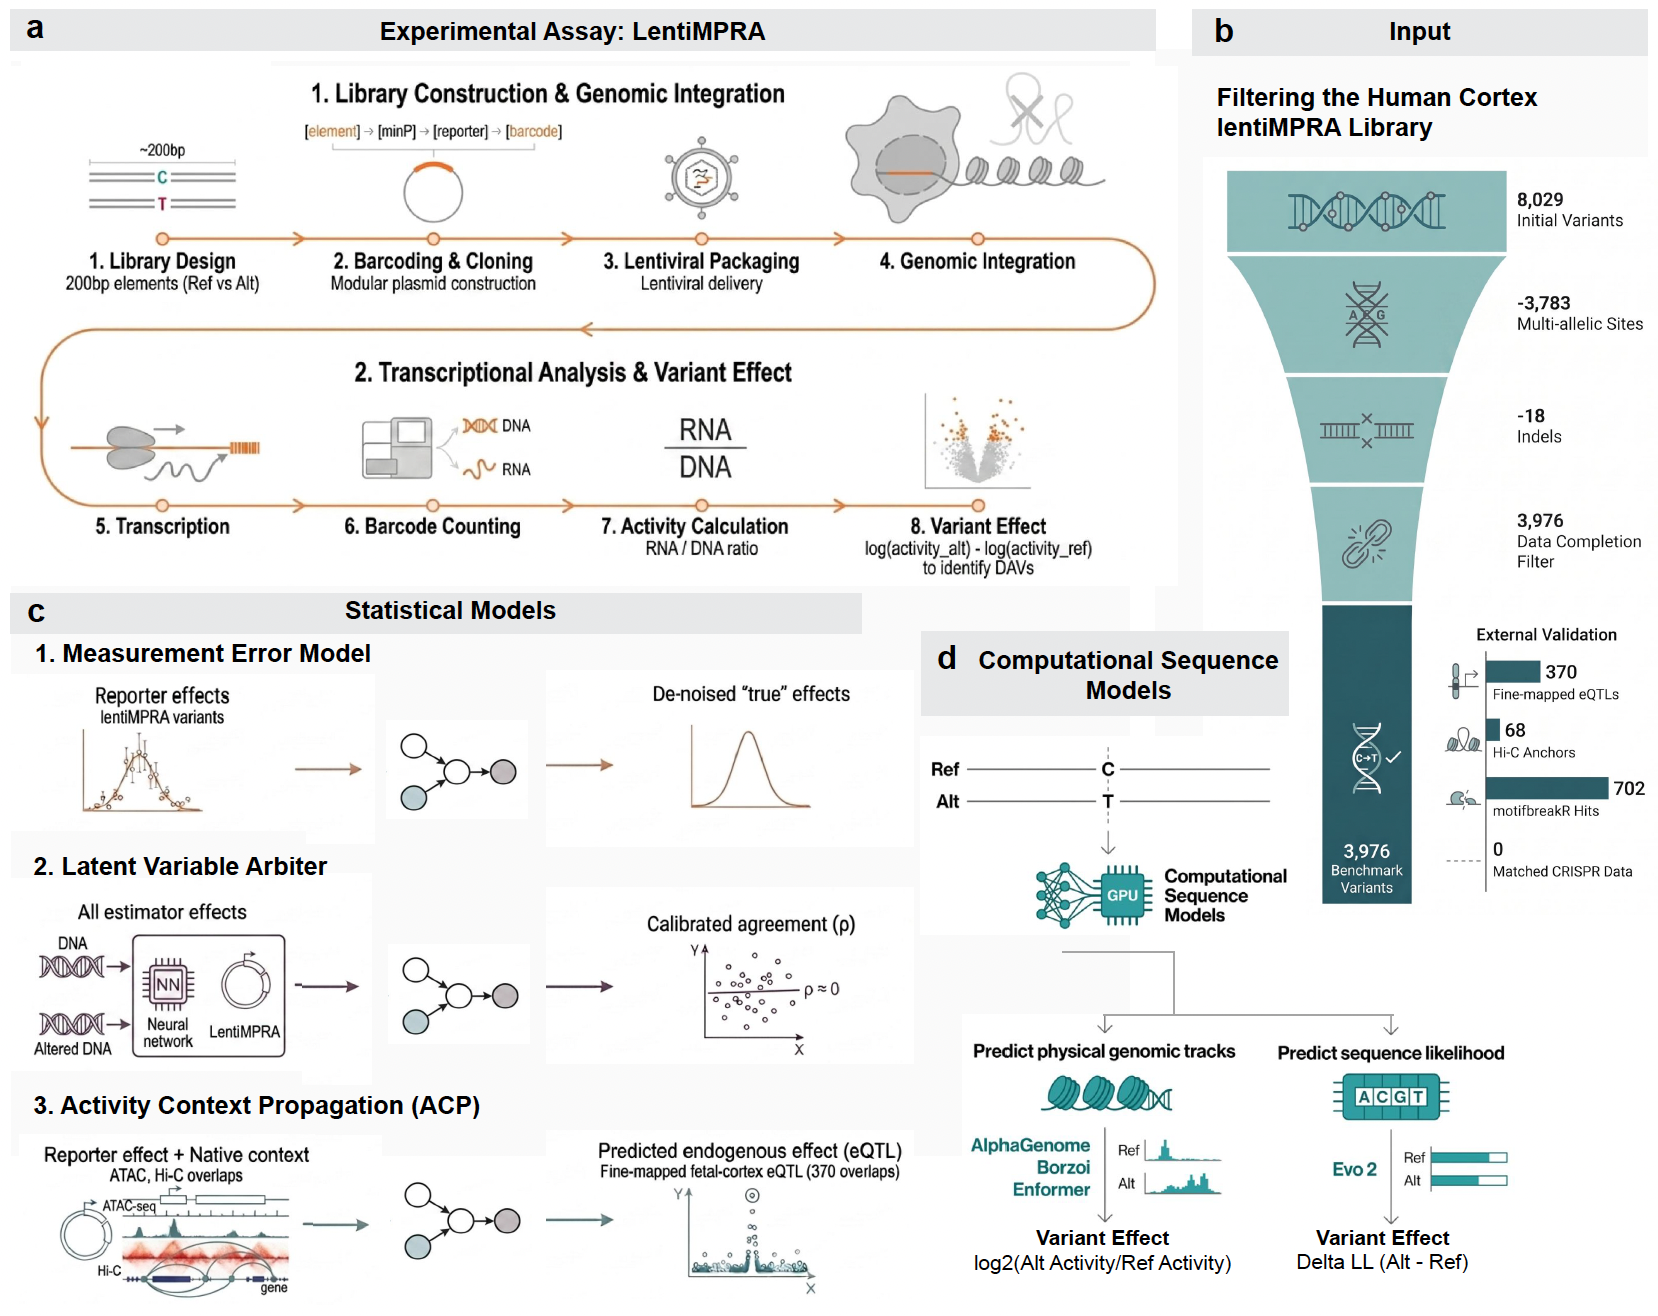
\includegraphics[width=\linewidth]{figures/fig1.png}
\caption{\textbf{Figure 1. Study overview: one variant set, two classes of estimator, and independent anchors.} (\textbf{a}) The lentiMPRA experimental assay: reference and alternate ~200 bp elements are barcoded, cloned, packaged into lentivirus, and integrated into developing-human-cortex chromatin; barcoded transcription is sequenced and a variant's reporter effect is log(activity\textsubscript{alt}) - log(activity\textsubscript{ref}), where activity is the RNA/DNA barcode ratio. (\textbf{b}) Filtering of the published cortex lentiMPRA library to the benchmark set: 8,029 initial variants, minus 3,783 multi-allelic sites and 18 indels, then a data-completeness filter, giving 3,976 biallelic single-nucleotide variants (76 differentially active). External coverage of this set: 370 in fine-mapped eQTL credible sets, 68 in Hi-C loop anchors, 702 with motifbreakR annotation, and 0 in any matched single-base CRISPR screen. (\textbf{c}) The three Bayesian models, each as input, model, and output: a measurement-error model (de-noised effects), a latent-variable model (calibrated agreement $\rho$), and an Activity-Context-Propagation model (predicted endogenous eQTL effect). (\textbf{d}) In silico scoring: for each variant the reference and alternate sequences are scored by the computational models; AlphaGenome, Borzoi, and Enformer return a change in predicted genomic-track activity (log\textsubscript{2} alt/ref), whereas the genomic language model Evo 2 returns a change in sequence likelihood ($\Delta$LL, alt - ref).}
\label{fig:fig1}
\end{figure*}


\section{Results}


\subsection{Model and reporter variant effects are uncorrelated, and the disagreement is not measurement noise}

If a foundation model and a reporter assay measured the same regulatory quantity, their variant effects would correlate. They do not. Across the 3,976 variants (Figure 1), AlphaGenome and Borzoi predicted effect magnitudes are uncorrelated with the lentiMPRA effect (Spearman $\rho$ = -0.02; sign concordance 0.50, at chance), and the disagreement does not concentrate where the reporter is most confident: on the 76 differentially active variants (DAVs, the reporter's own high-confidence hits) the correlation is if anything slightly negative ($\rho$ = -0.13), and the models recover DAVs barely above chance (AUROC 0.54; Figure 2a).

A skeptic's first objection is that reporter noise alone could erase a real correlation. It does not. A hierarchical Bayesian measurement-error model (regularized-horseshoe prior on the true effect, the measured limma standard error as known per-variant noise; Methods, Figure S3a) de-noises the reporter and reweights by reliability; the model-reporter agreement remains at zero (denoised $\rho$ $\approx$ 0; Figure 2b). The two instruments are not a noisy version of one measurement. They are measuring different things.

\begin{figure*}[t]
\centering
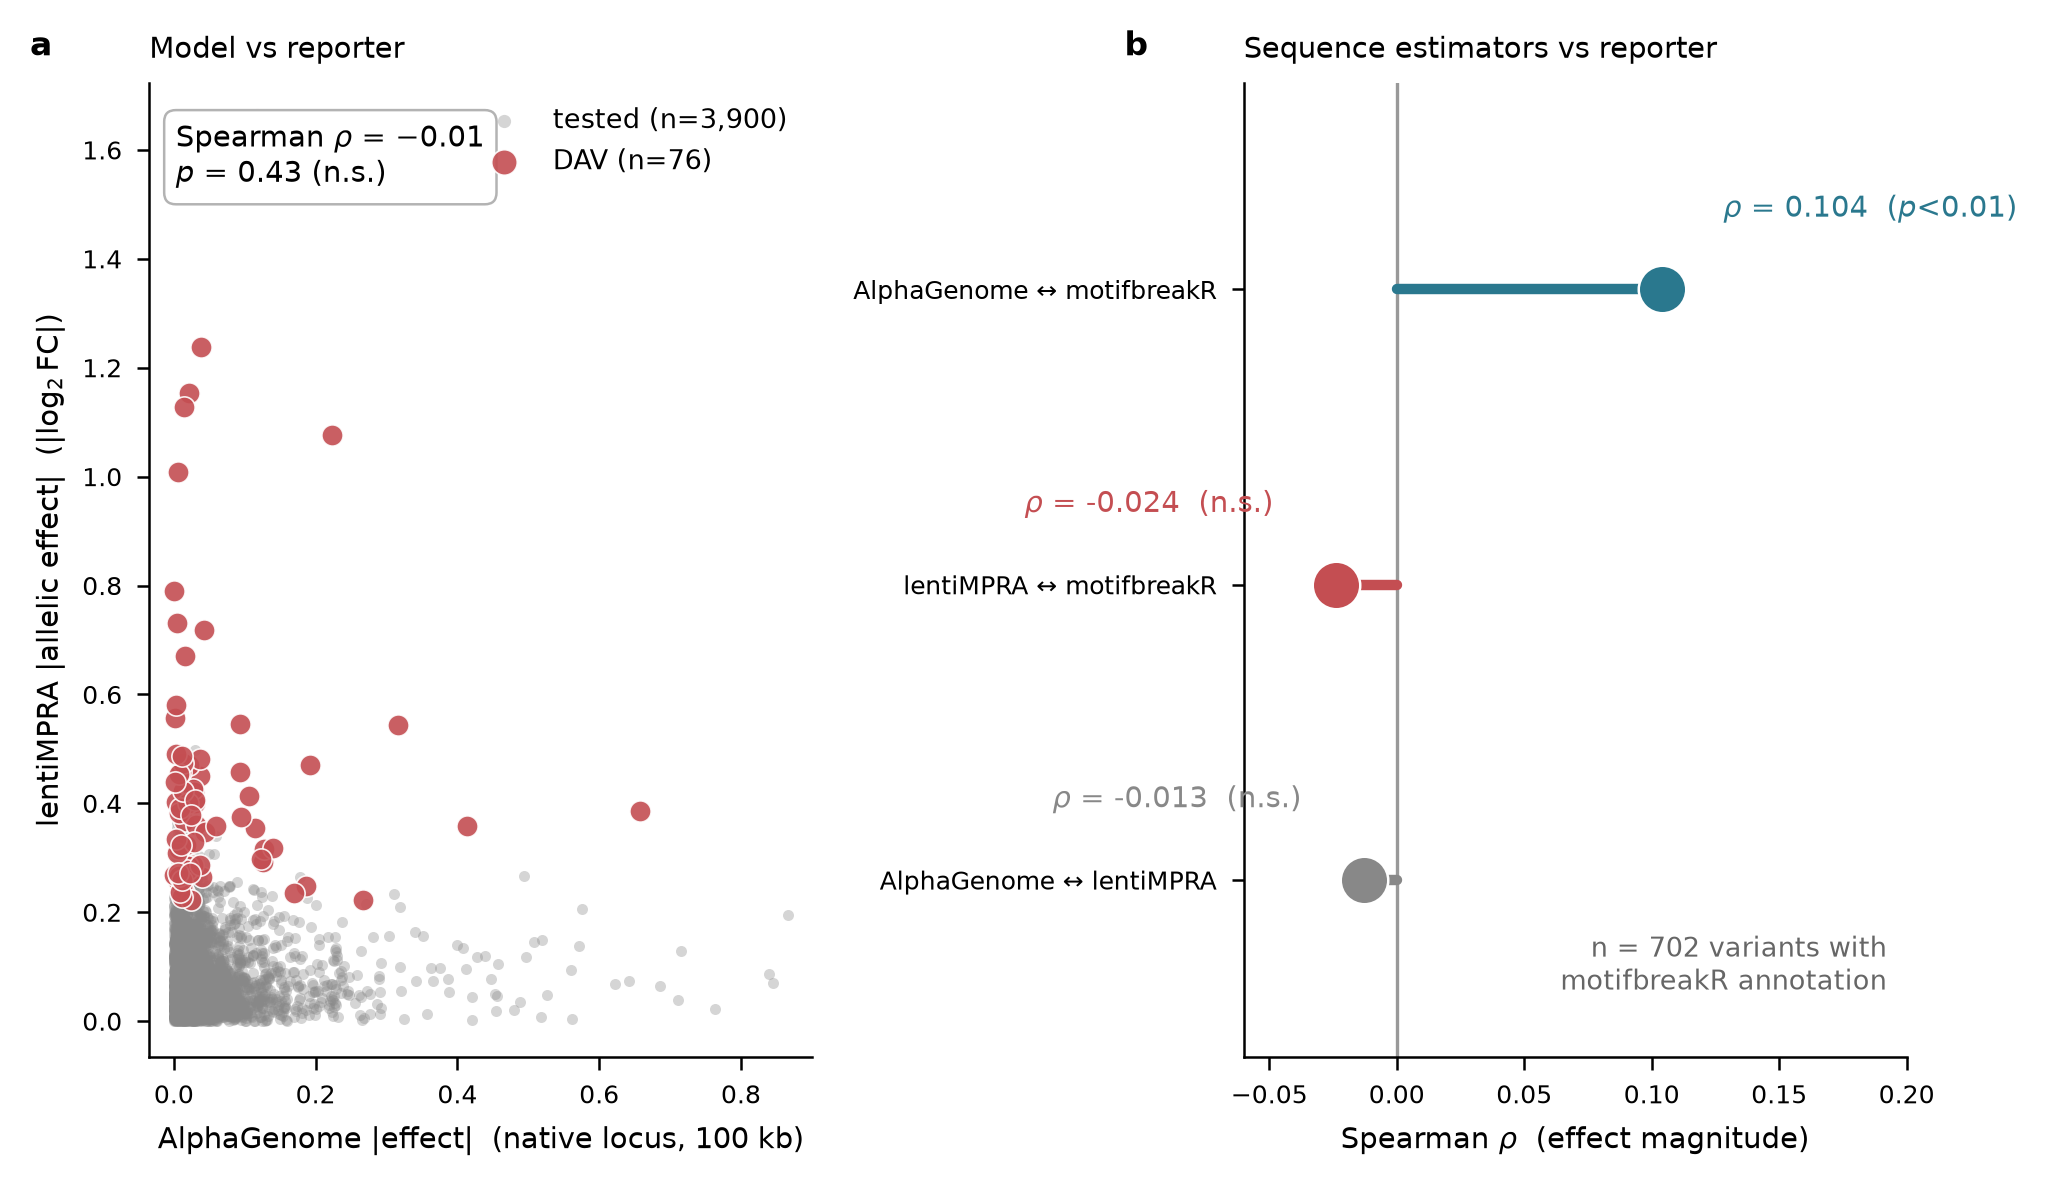
\includegraphics[width=\linewidth]{figures/fig2.png}
\caption{\textbf{Figure 2. Model and reporter effects are uncorrelated and the gap is not reporter noise.} (\textbf{a}) AlphaGenome effect magnitude versus lentiMPRA effect over 3,976 variants (76 DAVs highlighted); no relationship ($\rho$ = -0.02). (\textbf{b}) After Bayesian de-noising of the reporter, the model-reporter agreement is still zero, so the reported per-variant uncertainty does not explain it.}
\label{fig:fig2}
\end{figure*}


\subsection{The models agree with one another and with endogenous genetics; the reporter captures variation largely orthogonal to the model cluster}

Near-zero agreement could mean the models are simply uninformative. The multi-estimator structure says otherwise. The three activity-predicting models rank-agree strongly with one another (a sequence-level cluster: AlphaGenome-Borzoi $\rho$ = 0.55, Borzoi-Enformer $\rho$ = 0.81, AlphaGenome-Enformer $\rho$ = 0.58), and Enformer, run independently, reproduces both halves of the pattern (it tracks the other models and shows the same null agreement with the reporter, $\rho$ = -0.01, n.s.). Read across all five estimators of the same variants, agreement is not random but structured (Figure 3): the three models form a hot block and each tracks an independent fine-mapped eQTL anchor ($\rho$ = 0.24 to 0.28; Section 2.4), while the lentiMPRA correlates with none of them (|$\rho$| $\le$ 0.03).

Not every sequence model belongs to this cluster, and the exception is instructive. Evo 2, a genomic language model that scores sequence likelihood rather than regulatory activity, measures a distinct quantity: its per-variant likelihood change correlates with nothing else (vs. AlphaGenome $\rho$ = 0.005, vs. the reporter $\rho$ = 0.002, vs. the eQTL $\rho$ = 0.03; magnitudes ~100$\times$ larger, median |$\Delta$LL| = 1.01). "Sequence model" is therefore not one estimand: only the activity-predicting family forms the cluster the reporter is absent from. The reporter thus captures variation largely orthogonal to the concordant, endogenous-context estimators.

\begin{figure}[t]
\centering
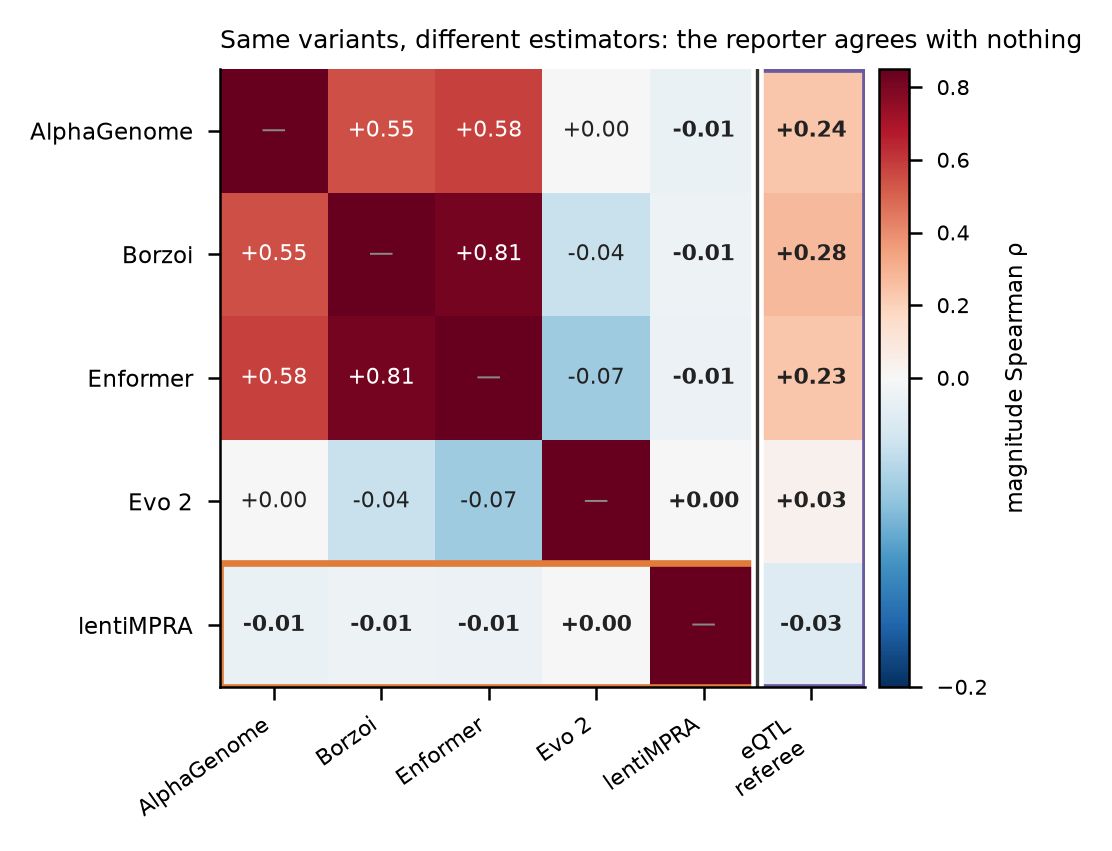
\includegraphics[width=0.66\linewidth]{figures/fig3.png}
\caption{\textbf{Figure 3. A structured cross-estimator discordance: the reporter agrees with nothing.} Pairwise magnitude Spearman $\rho$ among five estimators of all 3,976 variants, with an appended column for each estimator's agreement with the independent eQTL anchor (n = 370). The three activity models (AlphaGenome, Borzoi, Enformer) form a hot block and all track the eQTL; the integrated lentiMPRA and the likelihood model Evo 2 correlate with nothing. Diagonal omitted.}
\label{fig:fig3}
\end{figure}


\subsection{A calibrated latent-variable model, validated by simulation, places the agreement at zero}

Correlations on noisy observations understate or overstate the truth. To put a credible interval on the agreement itself, we fit a latent-variable generative model (NumPyro; Methods, Figure S3b): each variant has a latent endogenous effect and a latent assay effect drawn from a bivariate normal whose correlation $\rho$ is the calibrated model-reporter agreement, with AlphaGenome, Borzoi and motif disruption loading on the endogenous latent and the lentiMPRA on the assay latent (heteroscedastic by its measurement error). After separating each source's own noise from shared signal, the calibrated agreement is indistinguishable from zero ($\rho$ = -0.018, 95\% HDI [-0.064, +0.027]; Figure 4a).

The estimator is trustworthy: simulation-based calibration (data simulated at known $\rho$ and refit) recovers the truth with small bias ($\le$ 0.011) and nominal coverage (6/6, 17/20, 6/6 across $\rho$ = -0.3, 0, +0.3; 0 divergences; Figure S2), and the near-zero agreement is robust to model membership and loading choice, holding within |$\rho$| $\le$ 0.05 when motifbreakR is dropped, Enformer is added, or either CNN is left out (Figure S5). We therefore replace a per-variant verdict with a calibrated concordance map of all 3,976 variants (Figure 4b), decomposing them into four classes by which instrument moves: reporter-only (2,003), both-quiet (977), concordant (626), and endogenous-only (370). The near-zero concordance is uniform: it does not hide a responsive subset in any activity, conservation, or motif-disruption stratum.

\begin{figure*}[t]
\centering
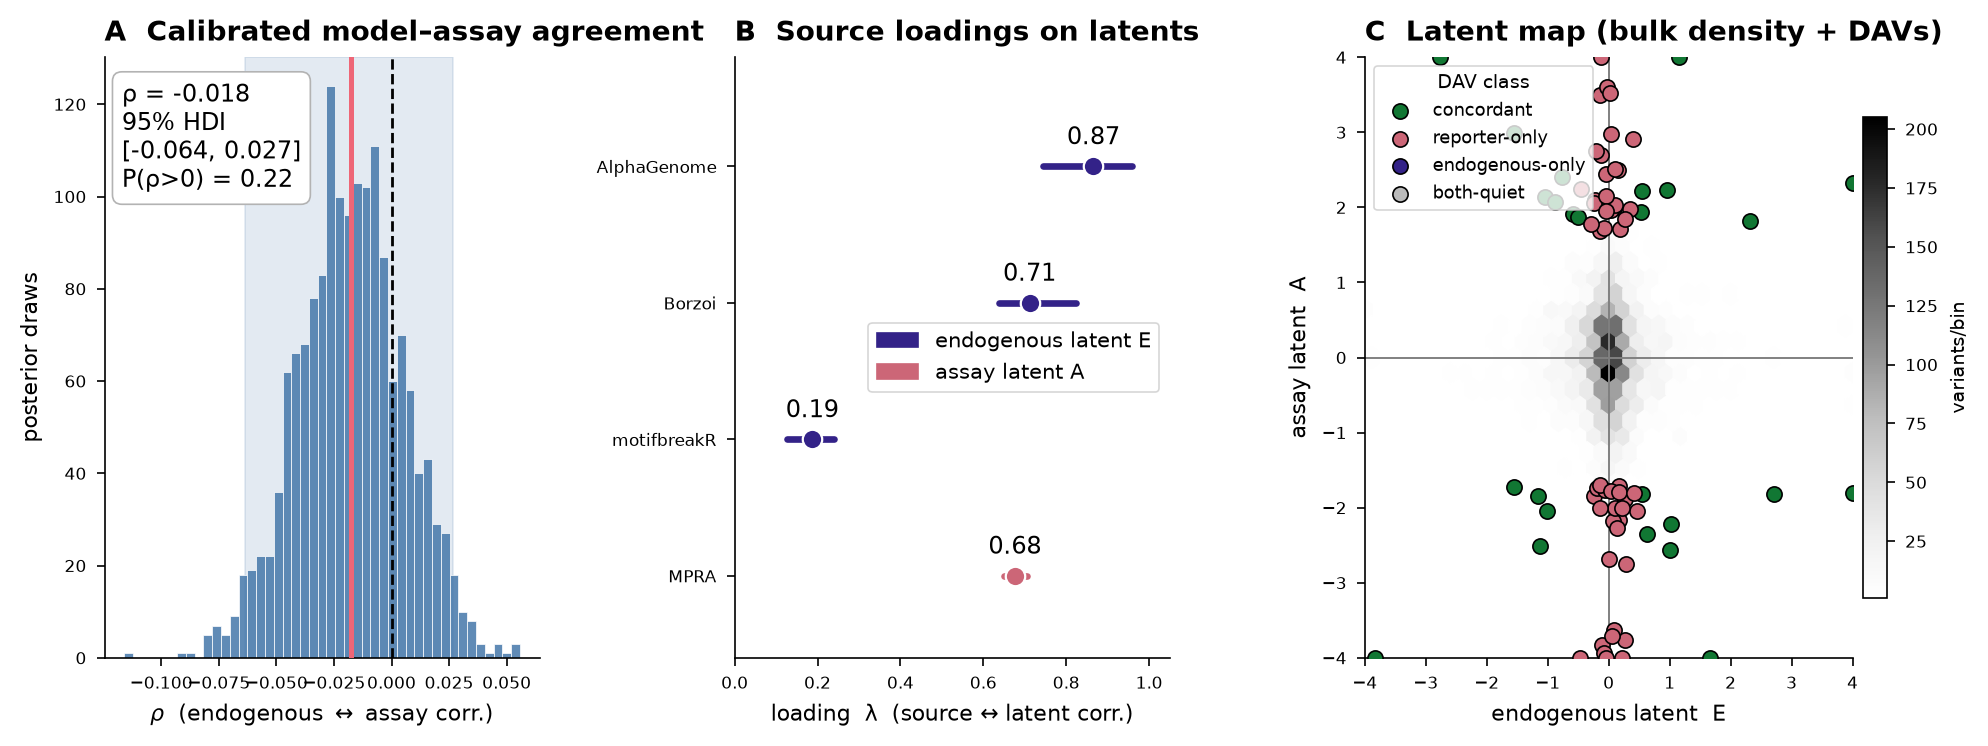
\includegraphics[width=\linewidth]{figures/fig4.png}
\caption{\textbf{Figure 4. A calibrated latent-variable model puts model-reporter agreement at zero.} (\textbf{a}) Posterior for the calibrated agreement $\rho$ after removing each source's noise; the 95\% HDI straddles zero. (\textbf{b}) Per-variant concordance map: the endogenous latent versus the assay latent, colored by attribution class (reporter-only, both-quiet, concordant, endogenous-only).}
\label{fig:fig4}
\end{figure*}


\subsection{An external endogenous anchor gives modest, independent support to the model ranking}

Because both instruments are in dispute, neither can adjudicate the other; a third, independent readout is required. We use a developmentally matched, fine-mapped fetal-cortex expression-QTL (eQTL) atlas: SuSiE credible sets with a per-variant posterior inclusion probability (PIP, the fine-mapping probability that a variant is causal) and a posterior effect size. Of the 3,976 variants, 370 fall in a credible set (25 at PIP $\ge$ 0.5). On this endogenous readout the models track the anchor and the reporter does not: AlphaGenome tracks the fine-mapped effect ($\rho$ = 0.24, 95\% CI [0.14, 0.33]) and Borzoi likewise ($\rho$ = 0.28), while the lentiMPRA does not ($\rho$ = -0.03, n.s.; Figure 5a).

The signal behaves as a real one should. Direction-of-effect concordance between AlphaGenome and the eQTL rises monotonically with causal confidence, from 50\% across all 370, to 60\% at PIP $\ge$ 0.1, to 80\% at PIP $\ge$ 0.5 (20/25, binomial p = 0.002; Figure 5b,c), and it is specific to the fine-mapped causal effect: it is near zero against the LD-contaminated lead-SNP z-score ($\rho$ = 0.001), which is why lead-SNP QTLs fail as benchmarks while fine-mapped ones succeed. A second, marginal-only cortex atlas (Walker 2019) shows the expected null (no tracking of the marginal signal), reinforcing that the agreement is a property of causal, credible-set effects. We present this as corroborating, not decisive: it rests on 370 variants (25 at high PIP). The reading is not that the models are right and the reporter wrong, but that an orthogonal endogenous readout aligns with the models, which is most parsimoniously an estimand mismatch. This recapitulates, with an independent instrument, the reporter-endogenous discordance the source lentiMPRA study already reported (55\% direction sharing with PsychENCODE eQTLs; r = 0.14).

\begin{figure*}[t]
\centering
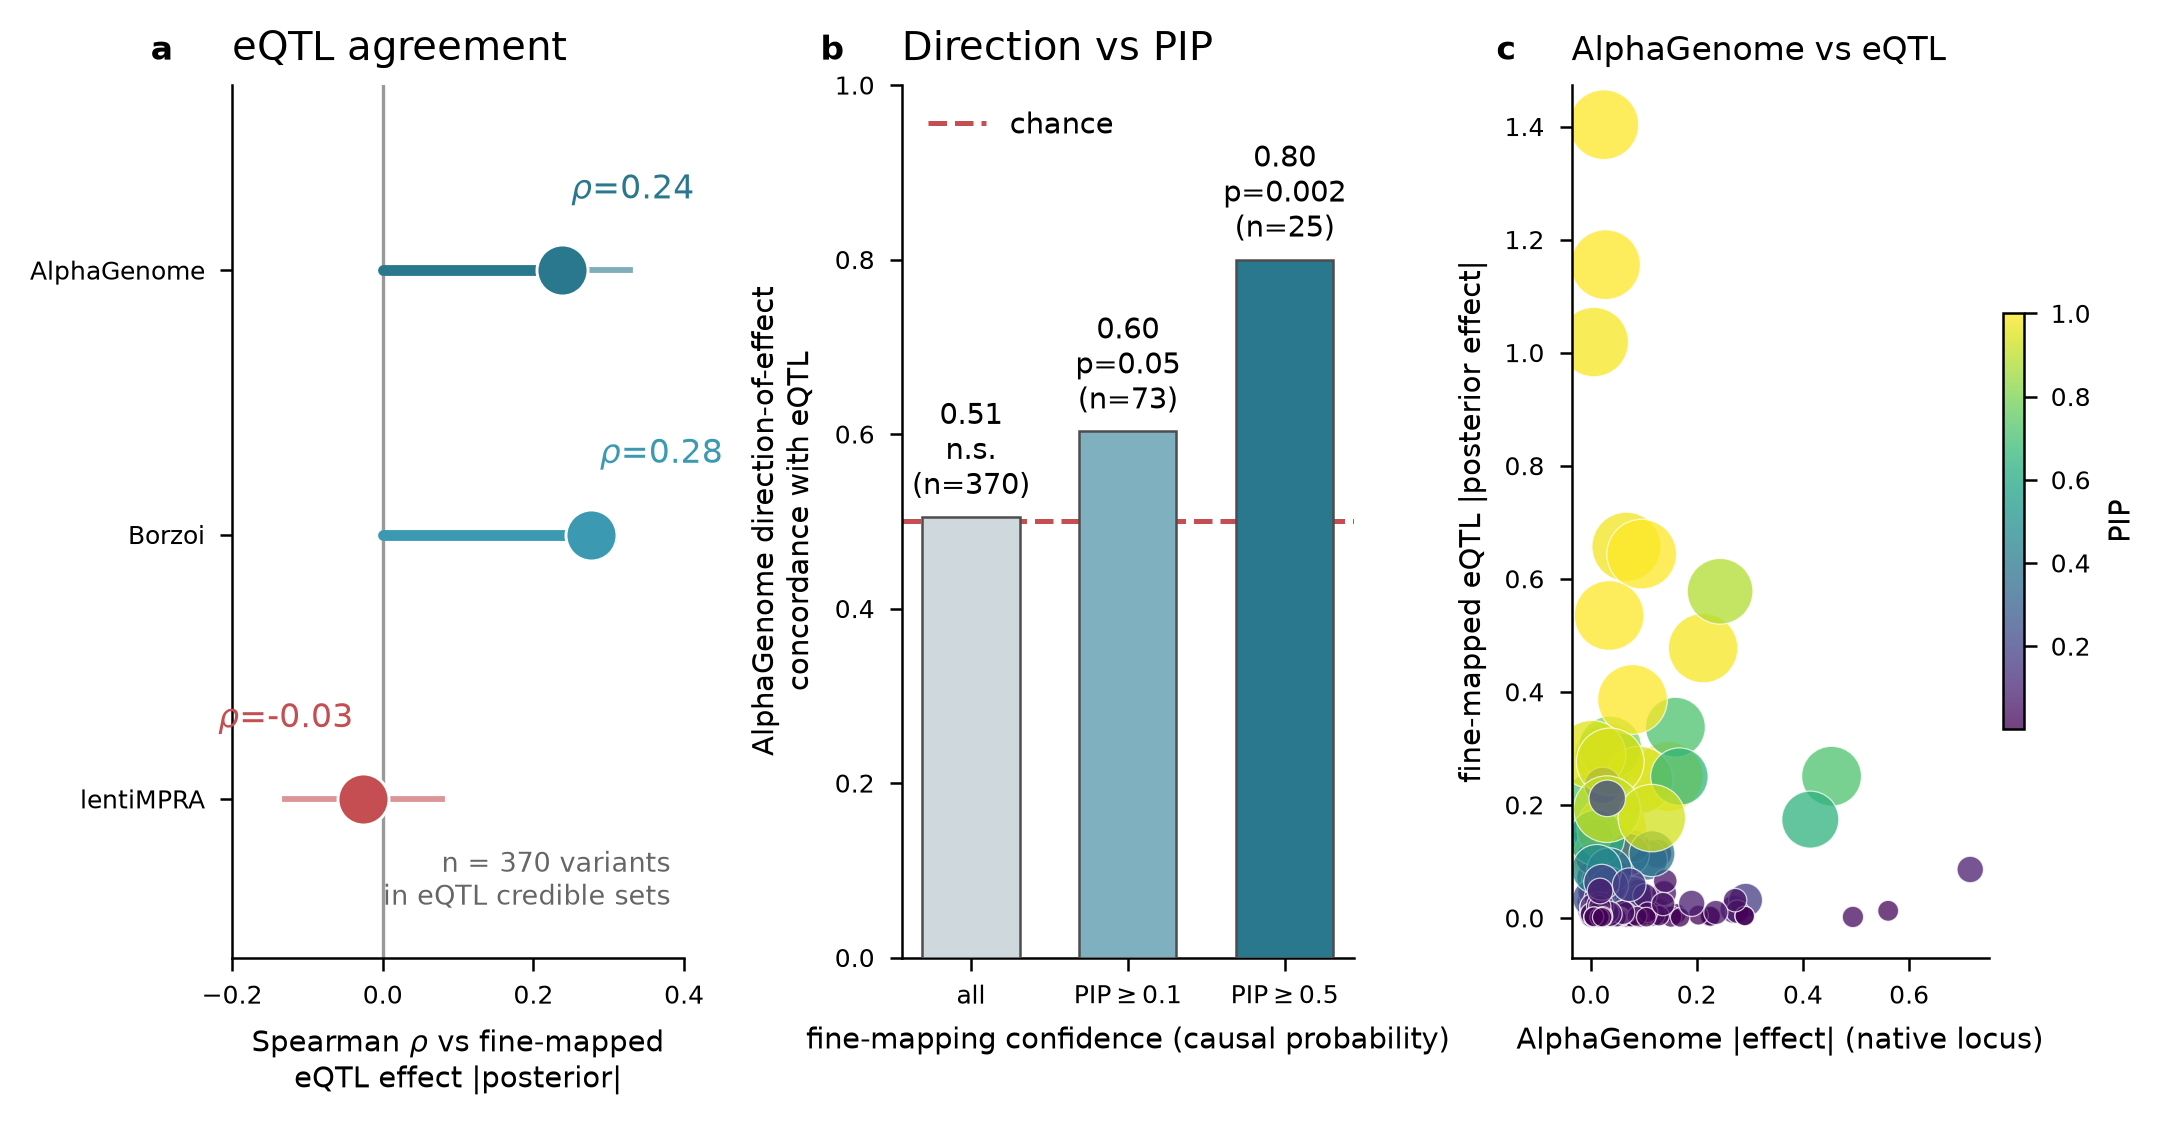
\includegraphics[width=\linewidth]{figures/fig5.png}
\caption{\textbf{Figure 5. An external fine-mapped eQTL anchor gives modest, independent support to the model ranking.} (\textbf{a}) Agreement of effect magnitude with the fine-mapped eQTL posterior effect for AlphaGenome, Borzoi and the lentiMPRA (n = 370; 95\% bootstrap CI). Both models agree; the reporter does not. (\textbf{b}) AlphaGenome direction concordance with the eQTL rises from chance to 80\% as PIP increases. (\textbf{c}) AlphaGenome effect versus fine-mapped eQTL posterior effect, sized by PIP.}
\label{fig:fig5}
\end{figure*}


\subsection{The gap is concentrated in the reporter-active, endogenously silent class}

If the disagreement reflects an estimand mismatch rather than a failure of either instrument, the largest divergences should fall where native context is most likely to matter and the decontextualized reporter is least able to see it. Two lines of evidence are consistent with this, and a third is exploratory. First, the mismatch is about context type, not context-window length: enlarging the model input from 100 kb to 1 Mb changes nothing (cross-context $\rho$ = 0.994), so the reporter is not missing signal the model would recover with more sequence, it is missing the native genomic context that the model approximates from the surrounding sequence. Second, an Activity-Context-Propagation (ACP) model built on the 370 fine-mapped pairs (Methods, Figure S3c) tested whether reporter potential reaches endogenous expression where context is favorable: it does not at this sample size. No model in the ladder beats an intercept null, the reporter$\times$context interaction is a coin flip ($\gamma$ = 0.001, 95\% CI [-0.056, +0.068]), and intrinsic scatter dominates. The dominant class is latent potential (reporter-active, endogenously silent; n = 34), which the measured context axes do not explain (Figure 6).

Third, as an exploratory observation, we intersected the variants with a Hi-C atlas of chromatin loops in induced neurons; 68 fall in loop anchors (all linkage-disequilibrium proxies, no lead SNPs). Within this small subgroup the reporter is attenuated (median |effect| 0.043 vs 0.064 elsewhere, p = 0.007) while the models are not (p = 0.32), baseline activity is matched (p = 0.44), and the model-reporter rank agreement, near zero elsewhere, rises to $\rho$ = +0.28 (bootstrap 95\% CI [+0.06, +0.48]; loop-versus-rest permutation p = 0.005; Figure S4). We do not interpret this as the two estimands sampling the same regulatory contact: an ectopically integrated reporter does not experience the native loop. The subgroup is small and defined post hoc, and the shift could equally reflect sequence composition, variant ascertainment, regulatory architecture, or sampling variation; it would need replication in an independent loop dataset before any mechanistic reading. We report it as a hypothesis-generating signal, not as support for the estimand-mismatch account.

\begin{figure*}[t]
\centering
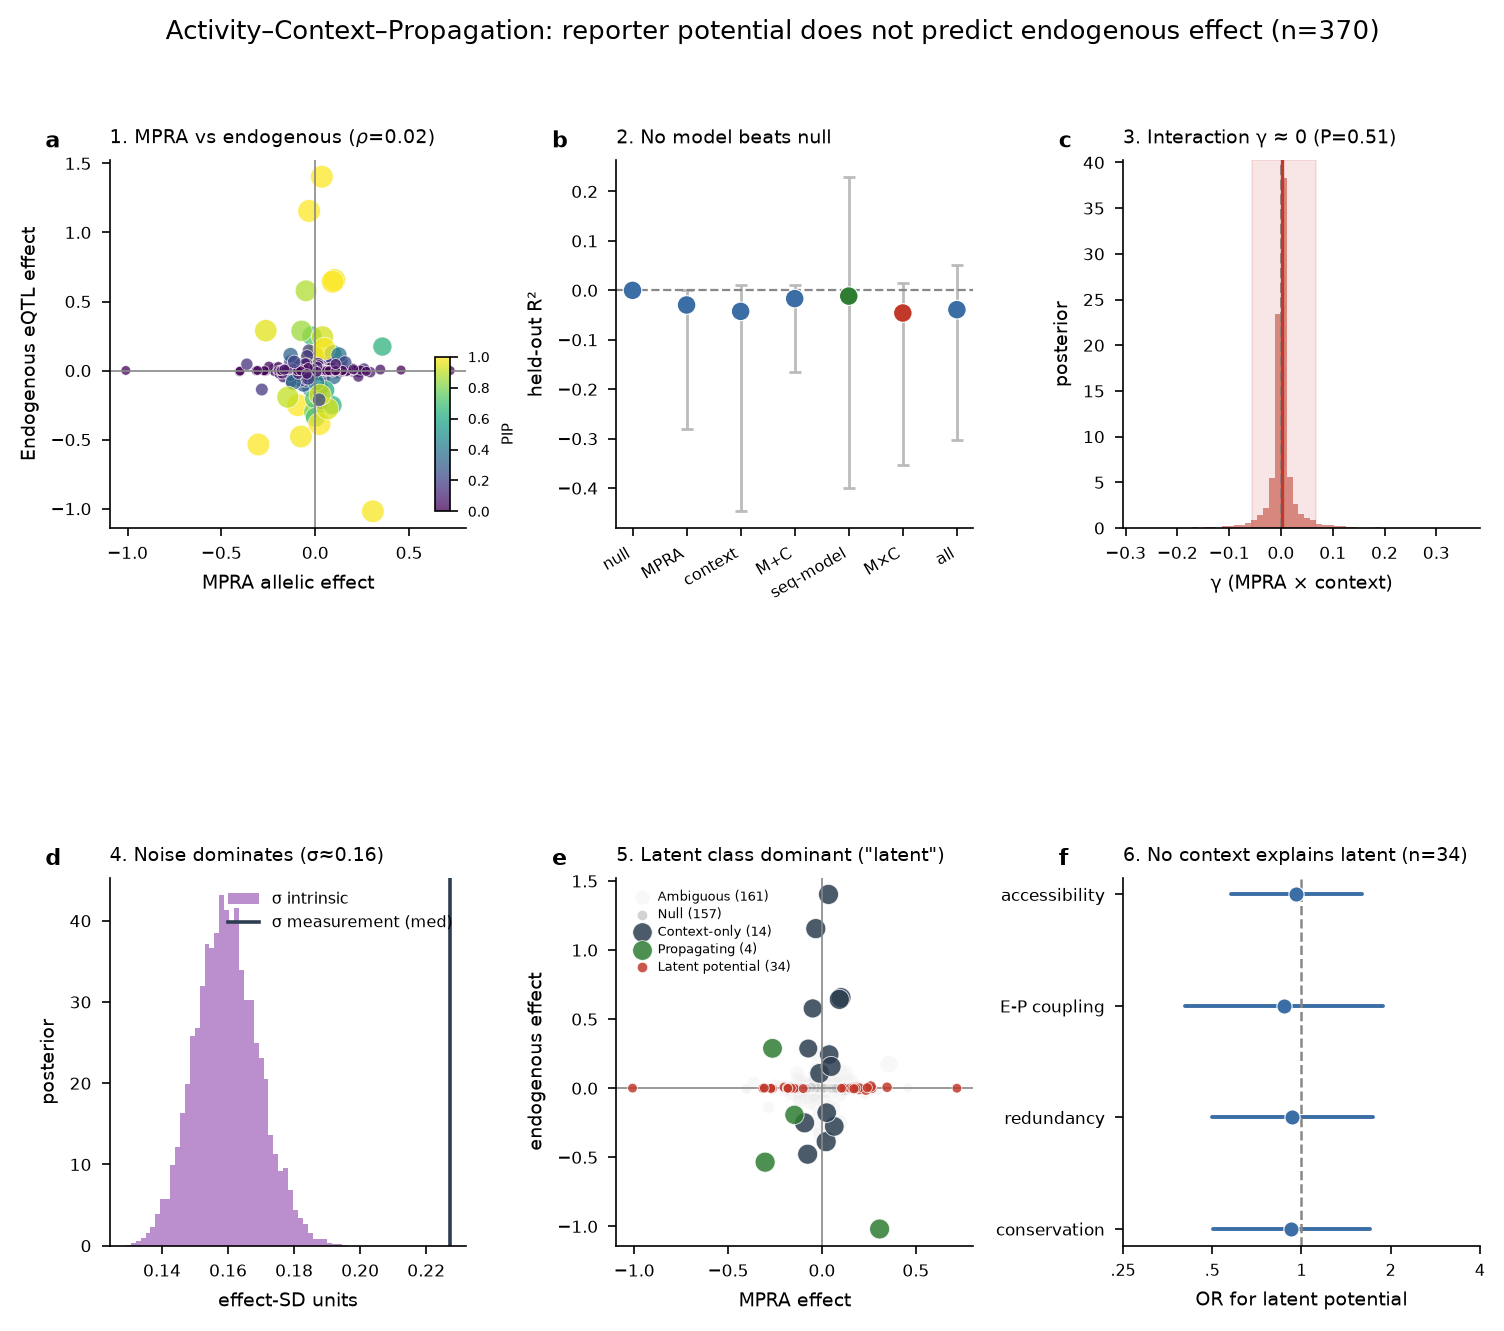
\includegraphics[width=\linewidth]{figures/fig6.png}
\caption{\textbf{Figure 6. The disagreement is concentrated in the reporter-active, endogenously silent class.} Activity-Context-Propagation (ACP) model on the 370 fine-mapped pairs: reporter potential does not propagate to the fine-mapped endogenous effect. No model in the nested ladder beats an intercept null, the reporter$\times$context interaction is negligible ($\gamma$ = 0.001, 95\% CI [-0.056, +0.068]), and an intrinsic-scatter term absorbs most of the variance. The dominant class is reporter-active but endogenously silent (n = 34), which the measured context axes do not explain.}
\label{fig:fig6}
\end{figure*}


\subsection{The concordance map prioritizes experiments, and defines a falsification test}

The concordance map is a decision tool, not only a diagnostic. Its concordant core is the sharpest place to ask what an endogenous experiment would show. We examined the 25 concordant DAVs (including the two largest allelic effects), resolving the signed direction of effect across lentiMPRA, AlphaGenome, Borzoi and, where available, the eQTL. Magnitude concordance only weakly predicts direction concordance: just 10 of 25 show three-way direction agreement (Figure 7a), consistent with the whole-set $\rho$ $\approx$ 0. One variant, rs76980967 (near MFGE8), is the single case where all four estimators agree in direction and it sits in a fine-mapped credible set (PIP = 0.64); we use it and rs2154984 (near STIP1) below only as illustrative variant evidence cards, not as therapeutic claims.

The more useful output is a ranked list of experiments. The map partitions variants into four classes (concordant; model-supported, reporter-quiet; reporter-supported, model-quiet; both-quiet), and the classes make divergent predictions for a native-locus edit, so measuring a matched panel across them would discriminate the competing explanations directly (Figure 7b). Under an estimand mismatch, a native edit at a model-supported, reporter-quiet variant should move endogenous expression while a reporter-supported, model-quiet variant should not; under model failure the pattern reverses; under shared measurement noise both are unstable across replicates. We therefore recommend selecting a small validation panel across the four classes, matched on baseline activity, measurement uncertainty, conservation, minor-allele frequency, and distance to the target gene, and editing representatives at the native locus in neural progenitors or cortical organoids by CRISPR base or prime editing. No matched single-base editing screen in this cell type yet exists, and a coordinate-and-allele intersection with public editing screens returned zero overlap with our set, so this panel is the natural next step and the one direct test that would falsify the estimand-mismatch reading.

\begin{figure*}[t]
\centering
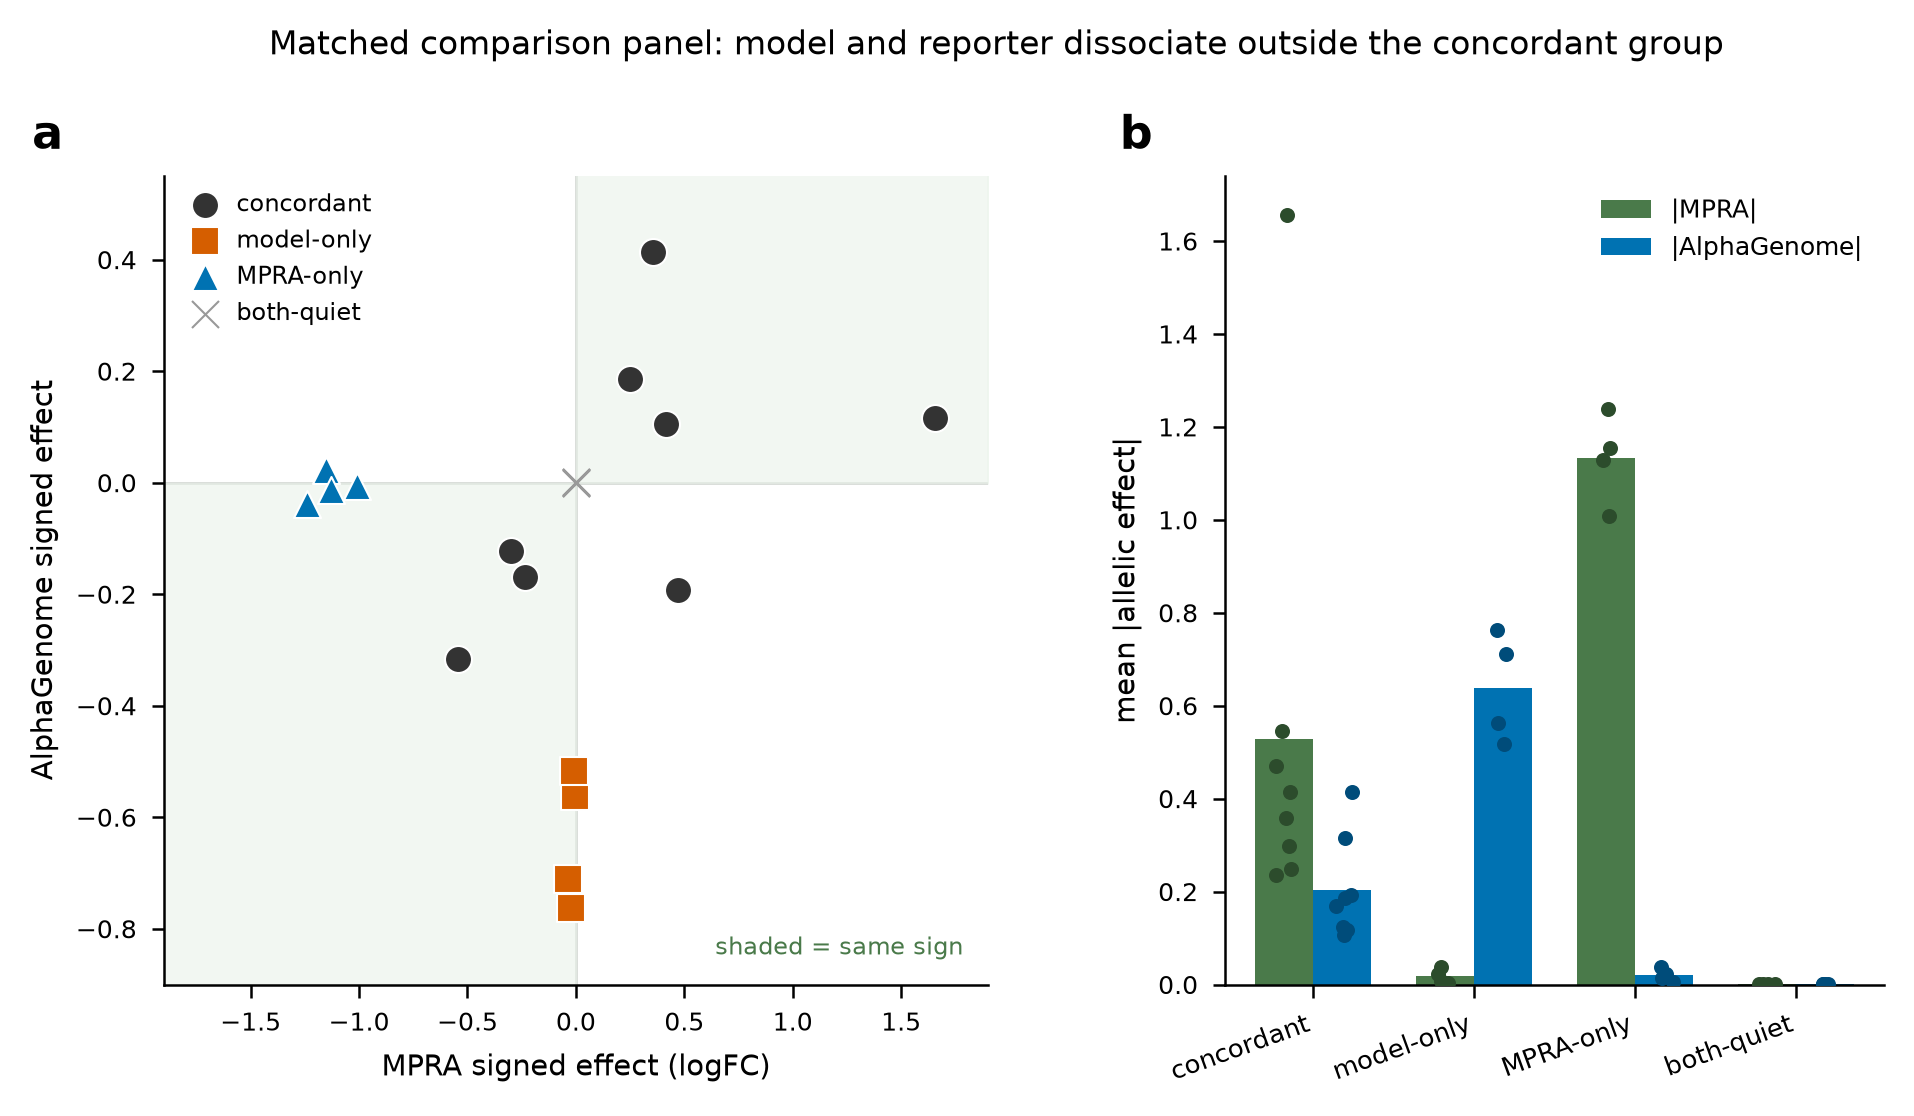
\includegraphics[width=\linewidth]{figures/fig7.png}
\caption{\textbf{Figure 7. The concordant core resolves direction of effect and prioritizes discriminating experiments.} (\textbf{a}) Signed direction of allelic effect per estimator for the 25 concordant DAVs, ranked by convergent-evidence score; only 10 show three-way agreement. (\textbf{b}) The four concordance classes and their divergent predictions for a native-locus edit, which define an information-maximizing validation panel; example evidence cards for rs76980967 (near MFGE8) and rs2154984 (near STIP1) are shown for illustration only.}
\label{fig:fig7}
\end{figure*}


\section{Discussion}

The central result is visible only when the comparisons are read together. Measured by five independent estimators, the same 3,976 variants show not random disagreement but a structured discordance (Figure 3): the three activity-predicting models cluster ($\rho$ = 0.55 to 0.81) and all track the fine-mapped eQTL ($\rho$ = 0.24 to 0.28), while the integrated lentiMPRA correlates with none of them (|$\rho$| $\le$ 0.03) and Evo 2 sits apart, scoring sequence likelihood rather than activity. This is not a reproducibility failure. Each instrument is internally sound, and the models' mutual agreement rules out the possibility that everything is noise. It is a category error to treat these as interchangeable readouts of one quantity. They estimate different physical quantities, so discordance is the expected consequence of an estimand mismatch, not evidence that any assay is wrong.

The external anchor is what makes this reading more than semantic. Because both instruments in the original comparison are in dispute, neither can adjudicate the other; a fine-mapped, developmentally matched eQTL atlas privileges neither, and it aligns with the models and not the reporter. That converts a symmetric "two instruments disagree" into an asymmetric one: the instrument that also agrees with independent endogenous genetics is the sequence model. The divergence is about context type, not context extent: a 100 kb and a 1 Mb receptive field agree at $\rho$ = 0.994, yet removing native flanking context altogether abolishes agreement. A more speculative, exploratory observation points the same way. In the small subgroup of variants at Hi-C loop anchors, model and reporter rankings become more similar ($\rho$ = +0.28 versus -0.02 elsewhere; Figure S4). We do not read this as the two instruments sampling the same physical contact, since an ectopically integrated reporter does not experience the native loop; the subgroup is small and defined post hoc, and the shift could reflect sequence composition or ascertainment. It is a hypothesis to test with an independent loop dataset, not evidence for the estimand-mismatch account.

This work is complementary to recent stress-tests of sequence models. Huang et al. and Sasse et al. documented that current models poorly explain cross-individual expression variation and often mispredict the direction of personal-genome effects, a performance gap against the correct endogenous estimand \cite{r17,r18}. Our contribution is orthogonal in kind: a benchmark can be mis-specified at the level of the estimand when the reference is a decontextualized reporter, and we provide a calibrated latent-variable framework plus an independent fine-mapped QTL anchor to diagnose it. The practical corollary is a recommendation. To benchmark in silico regulatory variant-effect prediction, a fine-mapped, developmentally matched endogenous QTL is a more closely aligned benchmark than a decontextualized reporter, and cross-instrument comparisons should be read as concordance maps between imperfect estimators, not as model-versus-truth scoreboards.

What the benchmark does not deliver is a mechanism for the divergence. The natural hypothesis, that reporter potential propagates to endogenous expression where native context is favorable, is not supported at this sample size: neither the reporter nor a reporter-by-context interaction predicts held-out endogenous effect, and an intrinsic-scatter term absorbs most of the variance. The descriptive content that survives is sharp: reporter-active but endogenously silent variants are the dominant class, so the divergence is concentrated, not diffuse. Powering its attribution, not the availability of a causal-base benchmark, is the rate-limiting step.


\subsection{Limitations}

The eQTL tie-breaker and the ACP analysis rest on 370 credible-set variants (25 at PIP $\ge$ 0.5), and the reporter-active, endogenously-silent class carries only 34 variants, so the ACP null is an absence of detectable context-dependence, not evidence of its absence. The benchmark is one lentiMPRA of 3,976 biallelic SNVs; the full exclusion funnel (17,069 to 15,335 to 8,029 to 3,976) removes variant classes the models cannot score rather than enriching for agreement, but the reduction is substantial and reported in full. Two similar models sharing training data partly inflates their mutual agreement; the latent-variable model isolates cross-source signal but cannot remove a shared prior, and because the models' training corpora may include brain tissue, part of the model-eQTL agreement could reflect shared signal (the fetal assay versus largely adult model tracks works against inflated agreement, not for it). The latent model is linear-Gaussian and captures monotone shared signal only. Finally, the most direct validation, a matched single-base CRISPR or prime-editing screen recreating these alleles in developing cortical cells, does not yet exist: public editing screens target coding or ClinVar variants in unrelated cell lines, and a coordinate-and-allele intersection returned zero overlap with our set. The 3D-genome convergence is correlational loop co-membership, not causal perturbation; a targeted editing screen at loop-anchored variants is the natural next step.


\section{Conclusion}

Treating a DNA foundation model and an MPRA as two imperfect estimators, rather than model versus truth, turns a null correlation from a disappointing benchmark result into an informative one. Across 3,976 psychiatric-risk regulatory variants, AlphaGenome and Borzoi agree with each other but not with an integrated developing-cortex lentiMPRA; the disagreement is not measurement noise; the calibrated agreement is credibly zero; and an independent, fine-mapped, developmentally matched eQTL benchmark tracks the models, not the reporter. The deliverable is a calibrated concordance map of where sequence prediction and reporter measurement encode the same signal, and a recommendationthat fine-mapped endogenous QTLs are a more closely aligned benchmark for in silico regulatory variant-effect prediction. Within the concordant core, magnitude concordance only weakly predicts sign agreement (10 of 25 concordant DAVs agree in direction), and the map turns this into a ranked set of discriminating experiments rather than a target list: a native-locus editing panel matched across the four concordance classes would test, and could falsify, the estimand-mismatch reading directly. The single variant on which the reporter, both models, and a fine-mapped eQTL all agree in direction, rs76980967 (near MFGE8), is the natural first evidence card for such a panel.


\section{Methods}


\subsection{Variant set and reporter measurements}

Variants and measured allelic effects were taken from the developing-human-cortex lentiMPRA of Deng et al. \cite{r1}, covering psychiatric-risk regulatory variants (brain eQTLs/caQTLs and GWAS SNPs) in primary cortical cells and hiPSC-derived cerebral organoids. The lentiMPRA reporter is lentivirally delivered and stably integrated into the host genome, with the assay signal restricted to integrated (chromatinized) copies. We used the study's processed per-variant log\textsubscript{2} fold change of alternate versus reference allele activity and its limma-moderated standard error and adjusted p-value. After QC (biallelic SNVs only; multi-allelic sites and indels excluded) the analysis set comprised 3,976 variants (hg38), of which 76 were differentially active (adjusted p $<$ 0.10; DAVs). A reference-allele check against hg38 (UCSC, Ensembl fallback) confirmed allele orientation on sampled variants.


\subsection{AlphaGenome and Borzoi variant scoring}

Variants were scored with AlphaGenome (v0.7.0, API) in native genomic context; per-variant summary is the mean allelic difference (DIFF_LOG2) over brain/CNS tracks pooled across four scorers (DNase, ATAC, CAGE, ChIP-histone), 100 kb window (1 Mb tested as ablation, cross-context $\rho$ = 0.994). Borzoi was run on GPU (524 kb windows) over brain DNase/CAGE/RNA tracks (reference-allele concordance 99.9\%). Both summaries are robust to the specific aggregation ($\rho$ $\ge$ 0.98).


\subsection{Independent fine-mapped eQTL benchmark}

As an external endogenous anchor we used the developing-brain xQTL atlas \cite{r14} (github.com/gandallab/devBrain_xQTL, Supplementary Data release, mixed cis-eQTL SuSiE fine-mapping), which provides per-variant credible-set membership, posterior inclusion probability (PIP), z-score and posterior effect size. Atlas coordinates (hg19) were lifted to hg38 with the UCSC hg19$\rightarrow$hg38 chain (122,016/122,050 variants lifted); 370 Deng variants matched an eQTL credible-set variant by exact chr:pos:ref:alt (0 required allele flip). Agreement was quantified with Spearman correlation of effect magnitude (95\% CI by bootstrap, 2,000 resamples) and with signed direction-of-effect concordance stratified by PIP (binomial test vs 0.5). Partial Spearman correlations controlled for phyloP, baseline activity and reporter effect by rank-regression residualization.


\subsection{Activity--Context--Propagation model}

The ACP analysis models the SuSiE posterior eQTL effect Y\textsubscript{i} (alt-oriented) from the oriented reporter effect M\textsubscript{i} and native context, using posterior SD as known measurement error and PIP as a causal-confidence weight. Context features (cortical ATAC accessibility across cell types, activity-by-contact enhancer--promoter contact breadth and target-gene count, phyloP, motifbreakR disruption, reporter baseline activity, and a library-wide enhancer-redundancy count) were split by provenance (AlphaGenome/Borzoi tracks excluded from the primary axes) and reduced within groups by PCA to orthogonal composites (accessibility, coupling, conservation) plus a redundancy axis, combined into one standardized context-favorability score approximately orthogonal to PIP (r = 0.06) and reporter magnitude (r = 0.03). A frequentist nested ladder (null; reporter; context; additive; reporter$\times$context; sequence-model; combined) was compared by repeated (5$\times$40) PIP-weighted k-fold cross-validation with ridge regression, reporting weighted held-out R$^2$ and paired win fractions. The Bayesian model, written in NumPyro, is Y\textsubscript{i} $\sim$ Normal($\mu$\textsubscript{i}, $\sigma$\textsubscript{i}) with $\mu$\textsubscript{i} = $\beta$\textsubscript{0} + $\beta$\textsubscript{M}M\textsubscript{i} + $\Sigma$\textsubscript{k}$\beta$\textsubscript{k}C\textsubscript{ik} + $\gamma$(M\textsubscript{i}$\times$fav\textsubscript{i}), a regularized-horseshoe prior on context coefficients and $\gamma$, a PIP-tempered likelihood ($\sigma$\textsubscript{meas,i} = posterior_SD\textsubscript{i}/$\sqrt{\phantom{x}}$PIP\textsubscript{i}), and an intrinsic-scatter term ($\sigma$\textsubscript{i}$^2$ = $\sigma$\textsubscript{meas,i}$^2$ + $\sigma$\textsubscript{extra}$^2$, $\sigma$\textsubscript{extra} $\sim$ HalfNormal(0.1)); inference used NUTS (4 chains, 1,500 warmup / 2,000 draws, target acceptance 0.95), with convergence by R-hat and effective sample size and fit by the standardized-residual distribution. Variants were classified into a 2$\times$2 of reporter status (DAV call or top-tertile magnitude with FDR $<$ 0.5) by endogenous status, the endogenous null defined from the posterior as P(|Y| $<$ $\delta$ | data) $>$ 0.8 at $\delta$ = 0.05. Context enrichment of the latent-potential class was tested against reporter-matched controls (nearest-neighbor matched on reporter magnitude, reporter uncertainty, PIP, activity and conservation) and by logistic regression of class membership on the context axes within the reporter-active pool.


\subsection{Context-window ladder}

For the context-type comparison (Section 2.5), AlphaGenome was additionally scored with a 1 Mb window (brain/CNS track mean, DIFF_LOG2) alongside the canonical 100 kb scoring. Agreement of each estimator's effect magnitude with the fine-mapped eQTL posterior-effect magnitude was computed by Spearman correlation with 95\% bootstrap confidence intervals (2,000 resamples) on the 369 credible-set variants carrying a 1 Mb score; the estimator-proximity matrix is the pairwise Spearman $\rho$ of the same magnitudes among the lentiMPRA, the two AlphaGenome windows and Borzoi. Cross-window agreement of the two AlphaGenome scorings was $\rho$ = 0.93 on this credible-set subset and $\rho$ = 0.99 genome-wide (all 3,976 variants).


\subsection{Bayesian measurement-error model}

Graphical models for all three probabilistic models are given in Figure S3. A hierarchical measurement-error model (NumPyro): measured effect y\textsubscript{i} ~ Normal($\theta$\textsubscript{i}, s\textsubscript{i}) with the limma standard error s\textsubscript{i} as known noise and a regularized horseshoe prior \cite{r9} on $\theta$\textsubscript{i}, fit non-centered by NUTS over all 3,976 variants (max R\textasciicircum{} = 1.007, no divergences). Posterior effects and inverse-variance weights were used to recompute agreement on denoised/reliability-weighted effects.


\subsection{Latent-variable generative model and simulation-based calibration}

A latent-variable model (NumPyro): each variant has two signed latents (E, A) drawn from a bivariate normal with unit variances and correlation $\rho$; AlphaGenome, Borzoi and motifbreakR load on E, the lentiMPRA (heteroscedastic, using its limma SE) on A. All sources z-scored so each loading equals its correlation with its latent; $\rho$ is identified through the cross-source covariance. Per-variant latents are marginalized analytically (linear-Gaussian core; Woodbury/matrix-determinant-lemma low-rank likelihood validated to 10\textsuperscript{-6} against a full multivariate normal), so NUTS samples only ~11 global parameters. Chains were run as independent single-chain fits (distinct seeds) and stacked for cross-chain R\textasciicircum{} (2 chains $\times$ 800 draws). phyloP was held out as orthogonal validation. Simulation-based calibration: data were simulated from the fitted model at a grid of known $\rho$ under the real heteroscedastic reporter noise and canonical loadings, then refit with the same model; we report HDI coverage and bias of the recovered $\rho$ across the grid.


\subsection{Additional sequence model (Enformer)}

To reduce dependence on the AlphaGenome/Borzoi family, we scored all 3,976 variants with Enformer (public "official-rough" weights, 197 kb receptive field), computing alternate-minus-reference predictions over central bins of brain CAGE and DNase tracks (single L40S GPU, 18 min; all 3,976 variants scored). Enformer is a third, independently developed sequence model with a distinct training regime; its inclusion tests whether the estimand mismatch is a property of sequence-to-function models in general rather than of two related architectures. Results are reported in Section 2.2 and Figure 3.


\subsection{Genomic language model (Evo 2)}

Evo 2 (7B parameters) was run on one NVIDIA L40S GPU. For each variant we extracted a 256 bp reference window centred on the variant from hg38 and constructed the alternate allele by substitution (100\% reference-base match across all 3,976 variants). Variant effect was the change in summed per-token log-likelihood, $\Delta$LL = LL(alt) - LL(ref); we report |$\Delta$LL| for magnitude comparisons. Because $\Delta$LL over a fixed window is a monotone rescaling of the mean per-token score, Spearman correlations are invariant to that choice; the tight window (versus an initial 1,024 bp window that diluted single-base effects to near zero) is what makes the per-variant values informative. Scoring used flash-attn 2.7.3 with the JIT cache staged on scratch.


\subsection{3D-genome loop overlap}

Chromatin-loop coordinates were taken from a published Hi-C atlas of three induced neuronal subtypes and iPSC in schizophrenia (Supplementary Table S4 of Ref. SCZ-3D), which lists, per loop anchor, the lead and LD-proxy (r$^2$ $>$ 0.1) risk SNPs assigned to that anchor. The table provides four anchor rsID columns (lead and LD-proxy for each of the two loop anchors); in this release the two lead-SNP columns are empty, so all 25,322 unique rsIDs derive from the two LD-proxy columns (13,660 and 13,478). We intersected them with our 3,976 variants by rsID, yielding 68 matches (all LD proxies; no lead SNPs; no differentially active variants). We emphasise that this table is a chromosome-conformation resource, not a CRISPR perturbation screen: the overlap identifies variants that share 3D-loop membership, not variants independently edited in cells. Loop-versus-rest comparisons used two-sided Mann--Whitney tests for absolute effect and baseline activity; model--reporter concordance used Spearman's $\rho$ with 2,000-fold bootstrap confidence intervals, and the loop-versus-rest $\rho$ difference was assessed by a 2,000-fold label permutation preserving the loop-set size.


\subsection{Concordant-core case study and prioritization}

The 25 concordant differentially active variants were taken as the intersection of the calibrated concordant class with the differential-activity call. For each we recorded the signed allelic effect of the lentiMPRA (log\textsubscript{2} fold change and its horseshoe-shrunk posterior mean), AlphaGenome (canonical brain summary), Borzoi (brain-track signed mean), and, where available, the fine-mapped eQTL posterior effect; all were oriented to the alternate allele. Direction agreement was scored across the reporter and the two foundation models (all-agree, two-of-three, or models-oppose-reporter), and a fine-mapped eQTL direction was counted only for variants in a credible set with PIP $\ge$ 0.1 and a non-trivial posterior effect. The convergent-evidence score is the sum of seven bounded, equally-scaled axes (direction agreement, reporter effect magnitude and significance, fine-mapped eQTL support (credible-set membership, PIP tier, and signed agreement), psychiatric-GWAS linkage-disequilibrium count across nine disorders, motifbreakR TF-motif disruption, AlphaGenome brain accessibility and reporter baseline activity, and phyloP conservation), each capped so no single axis dominates. Predicted target genes were assigned from activity-by-contact enhancer--gene links (per cortical cell type), fine-mapped eQTL target, and motifbreakR-disrupted TF, in that priority. The matched comparison panel comprised the 8 top-ranked concordant variants, the 4 model-only (endogenous-latent-active/reporter-quiet) variants with the largest AlphaGenome effect, the 4 reporter-only variants with the largest reporter effect, and the 4 lowest-effect both-quiet variants, drawn from the same calibrated classes and compared on baseline reporter activity.


\subsection{Target tractability and disease provenance}

For the genes nominated by the concordant core we queried the Open Targets Platform (GraphQL API v4) for target tractability (small-molecule, antibody, and PROTAC/degrader modality buckets), genetic constraint (gnomAD loss-of-function observed/expected upper bound, LOEUF), reported safety liabilities, and disease associations. Each modality was assigned a tier (clinical/structural evidence, medium-confidence annotation, or predicted only), and genes were ranked by a composite of causal-pointer strength (gene-link tier plus direction agreement), best modality tier, and maximum psychiatric/neurological disease-association score. Disease provenance of each variant was established from its Open Targets credible sets: a variant was assigned a genome-wide psychiatric indication if in linkage disequilibrium with a genome-wide-significant psychiatric GWAS signal in the reference panel, and otherwise classified by the strongest available credible set (sub-threshold psychiatric GWAS, brain molecular QTL only, non-psychiatric GWAS trait, or none). LOEUF, tractability tiers, and disease provenance are provided as a per-gene table.


\subsection{Orthogonal evidence and statistics}

Independent estimators: motifbreakR PWM motif-disruption scores \cite{r6}, phyloP conservation \cite{r7}, and the fine-mapped eQTL atlas \cite{r14}. Agreement by Spearman rank correlation (denoted $\rho$ throughout; \textit{p} denotes a p-value, never a correlation); class separation by Mann--Whitney U and AUROC; a subgroup scan over candidate strata was assessed against a permutation null. Analyses used Python (NumPy, pandas, SciPy) with NumPyro/JAX \cite{r8} and ArviZ. Coordinate liftover used pyliftover with the UCSC chain; SuSiE fine-mapping is as provided by the atlas \cite{r20}.


\subsection{Data and code availability}

Processed benchmark tables, model scores, the eQTL-overlap table, SBC results and all analysis scripts are provided as project artifacts with a pinned environment specification and fixed seeds. The full per-variant concordance map for all 3,976 variants (coordinates, each estimator's effect, and the calibrated posterior class probabilities (P\textsubscript{concordant}, P\textsubscript{reporter-only}, P\textsubscript{model-only}, P\textsubscript{both-quiet}) alongside the hard class call) is released as a documented supplementary table so downstream users can filter on posterior class probability rather than hard calls. Reporter measurements derive from Deng et al. \cite{r1}; the eQTL atlas from \cite{r14}.


\section{Reproducibility and Ethics}

\textbf{Reproducibility.} This is a secondary reanalysis of published data; no new human or animal data were generated. Reporter measurements are from Deng et al. \cite{r1}; the fine-mapped eQTL benchmark is the developing-brain xQTL atlas \cite{r14} (SuSiE credible sets). AlphaGenome was accessed via its API (v0.7.0); Borzoi and Enformer were run from public pretrained weights (Enformer "official-rough", scored on one GPU). All variant coordinates are hg38; the eQTL atlas (hg19) was lifted with the UCSC chain. Every analysis script was written from scratch for this study and is provided as project artifacts with a pinned environment; random seeds are fixed and reported, and MCMC diagnostics (R\textasciicircum{}, divergences) are reported for every fit.

\textbf{Ethics and data use.} No identifiable individual-level genotype or phenotype data were accessed; all inputs are aggregate/summary-level published resources. The AlphaGenome API terms govern redistribution of its outputs; we release derived per-variant effect summaries needed to reproduce the figures, not raw API responses. The variant library is ascertained for psychiatric-disorder-associated regulatory variants; we make no clinical or diagnostic claims about any variant, and the per-variant concordance map is a research triage, not a basis for clinical interpretation.

\section*{References}
\begin{thebibliography}{99}
\small
\bibitem[1]{r1} Deng C, Whalen S, Steyert M, et al. Massively parallel characterization of regulatory elements in the developing human cortex. Science 384, eadh0559 (2024). doi:10.1126/science.adh0559.
\bibitem[2]{r2} Avsec Ž, Agarwal V, Visentin D, et al. Effective gene expression prediction from sequence by integrating long-range interactions. Nature Methods 18, 1196–1203 (2021). doi:10.1038/s41592-021-01252-x.
\bibitem[3]{r3} Linder J, Srivastava D, Yuan H, Agarwal V, Kelley DR. Predicting RNA-seq coverage from DNA sequence as a unifying model of gene regulation. Nature Methods (2025); bioRxiv 2023.08.30.555582. doi:10.1101/2023.08.30.555582.
\bibitem[4]{r4} Kelley DR, Reshef YA, Bileschi M, et al. Sequential regulatory activity prediction across chromosomes with convolutional neural networks. \textit{Genome Research} 28, 739--750 (2018). doi:10.1101/gr.227819.117.
\bibitem[5]{r5} Tewhey R, Kotliar D, Park DS, et al. Direct identification of hundreds of expression-modulating variants using a multiplexed reporter assay. Cell 165, 1519–1529 (2016). doi:10.1016/j.cell.2016.04.027.
\bibitem[6]{r6} Coetzee SG, Coetzee GA, Hazelett DJ. motifbreakR: an R/Bioconductor package for predicting variant effects at transcription factor binding sites. Bioinformatics 31, 3847–3849 (2015). doi:10.1093/bioinformatics/btv470.
\bibitem[7]{r7} Pollard KS, Hubisz MJ, Rosenbloom KR, Siepel A. Detection of nonneutral substitution rates on mammalian phylogenies. Genome Research 20, 110–121 (2010). doi:10.1101/gr.097857.109.
\bibitem[8]{r8} Phan D, Pradhan N, Jankowiak M. Composable effects for flexible and accelerated probabilistic programming in NumPyro. arXiv 1912.11554 (2019). doi:10.48550/arXiv.1912.11554.
\bibitem[9]{r9} Carvalho CM, Polson NG, Scott JG. The horseshoe estimator for sparse signals. Biometrika 97, 465–480 (2010). doi:10.1093/biomet/asq017.
\bibitem[10]{r10} GTEx Consortium. The GTEx Consortium atlas of genetic regulatory effects across human tissues. Science 369, 1318–1330 (2020). doi:10.1126/science.aaz1776.
\bibitem[11]{r11} Avsec \v{Z}, et al. AlphaGenome: advancing regulatory variant effect prediction with a unified DNA sequence model. bioRxiv 2025.06.25.661532 (2025). doi:10.1101/2025.06.25.661532.
\bibitem[14]{r14} Cross-ancestry atlas of gene, isoform, and splicing regulation in the developing human brain. Science 384, eadh0829 (2024). Data: github.com/gandallab/devBrain_xQTL. doi:10.1126/science.adh0829.
\bibitem[15]{r15} Chen KM, Wong AK, Troyanskaya OG, et al. A sequence-based global map of regulatory activity for deciphering human genetics. Nature Genetics 54, 940–949 (2022). doi:10.1038/s41588-022-01102-2.
\bibitem[16]{r16} Zhou J. Sequence-based modeling of three-dimensional genome architecture from kilobase to chromosome scale. Nature Genetics 54, 725–734 (2022). doi:10.1038/s41588-022-01065-4.
\bibitem[17]{r17} Huang C, Shuai RW, Baokar P, et al. Personal transcriptome variation is poorly explained by current genomic deep learning models. Nature Genetics 55, 2056–2059 (2023). doi:10.1038/s41588-023-01574-w.
\bibitem[18]{r18} Sasse A, Ng B, Spiro AE, et al. Benchmarking of deep neural networks for predicting personal gene expression from DNA sequence highlights shortcomings. Nature Genetics 55, 2060–2064 (2023). doi:10.1038/s41588-023-01524-6.
\bibitem[19]{r19} Murphy D, Beardall W, Rei M, et al. Predicting cell type-specific epigenomic profiles accounting for distal genetic effects. Nature Communications 15, 10510 (2024). doi:10.1038/s41467-024-54441-5.
\bibitem[20]{r20} Wang G, Sarkar A, Carbonetto P, Stephens M. A simple new approach to variable selection in regression, with application to genetic fine mapping. J. R. Stat. Soc. B 82, 1273–1300 (2020). doi:10.1111/rssb.12388.
\end{thebibliography}

\section*{Supplementary Figures}
\setcounter{figure}{0}
\renewcommand{\thefigure}{S\arabic{figure}}
\begin{figure*}[t]
\centering
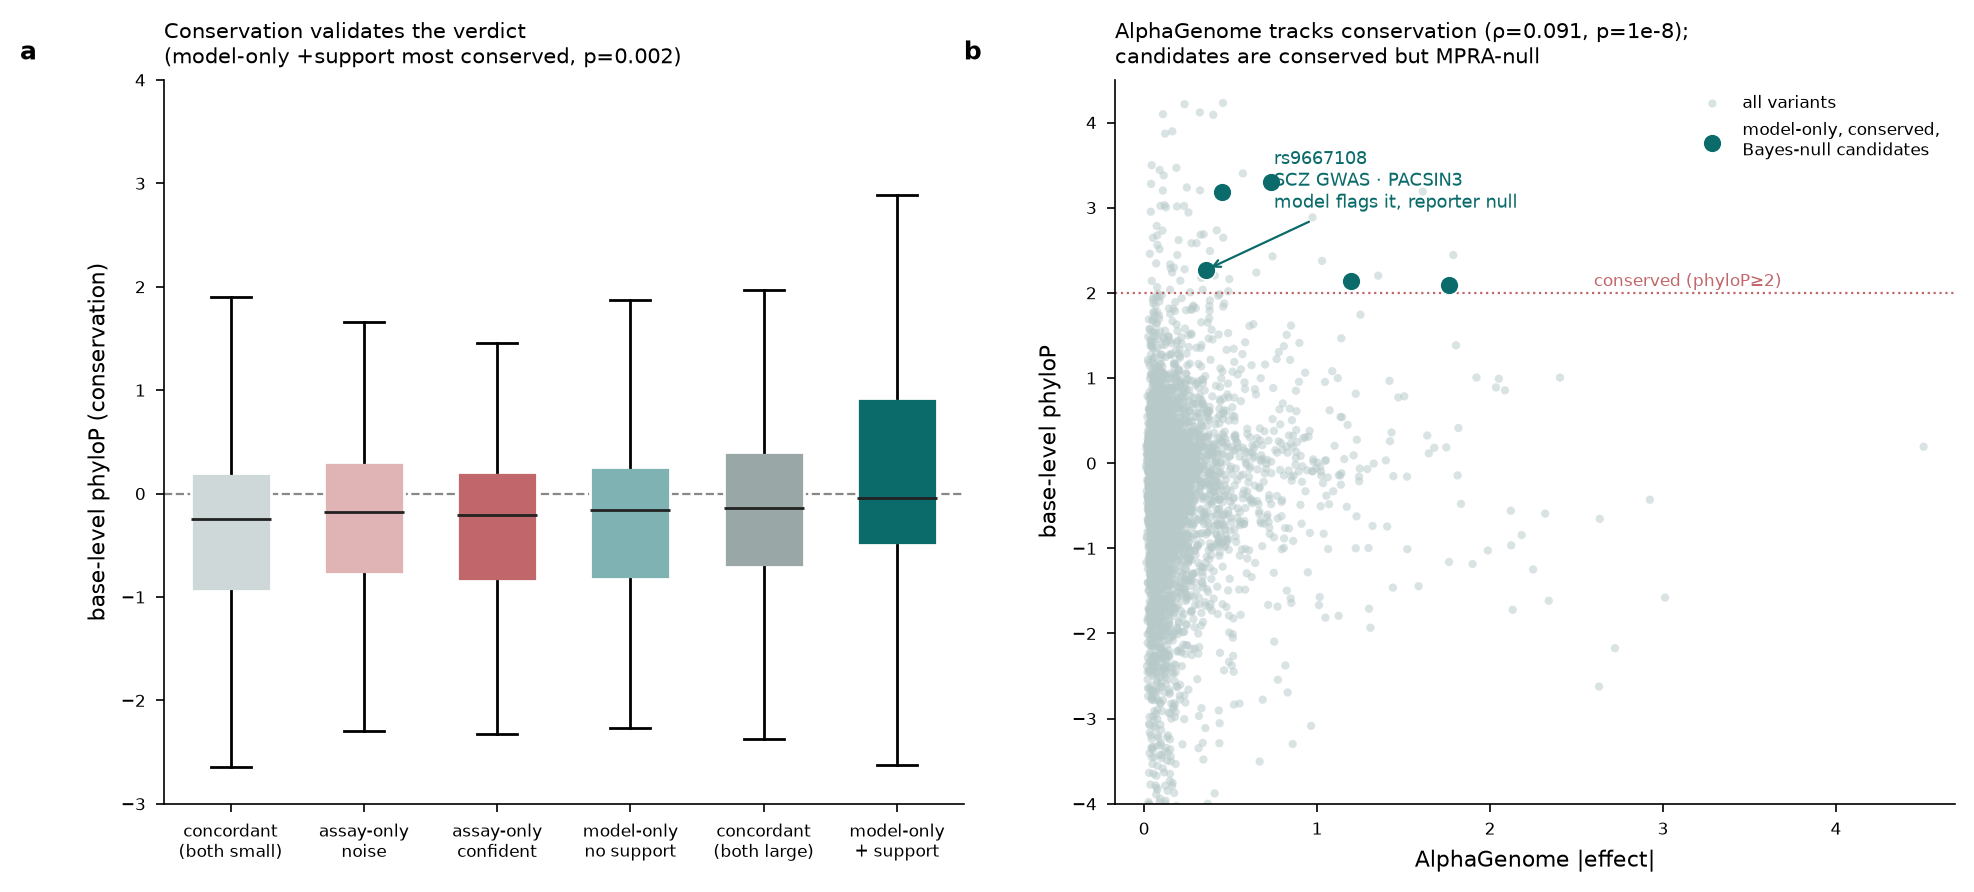
\includegraphics[width=0.49\linewidth]{figures/figS1a.png}\hfill
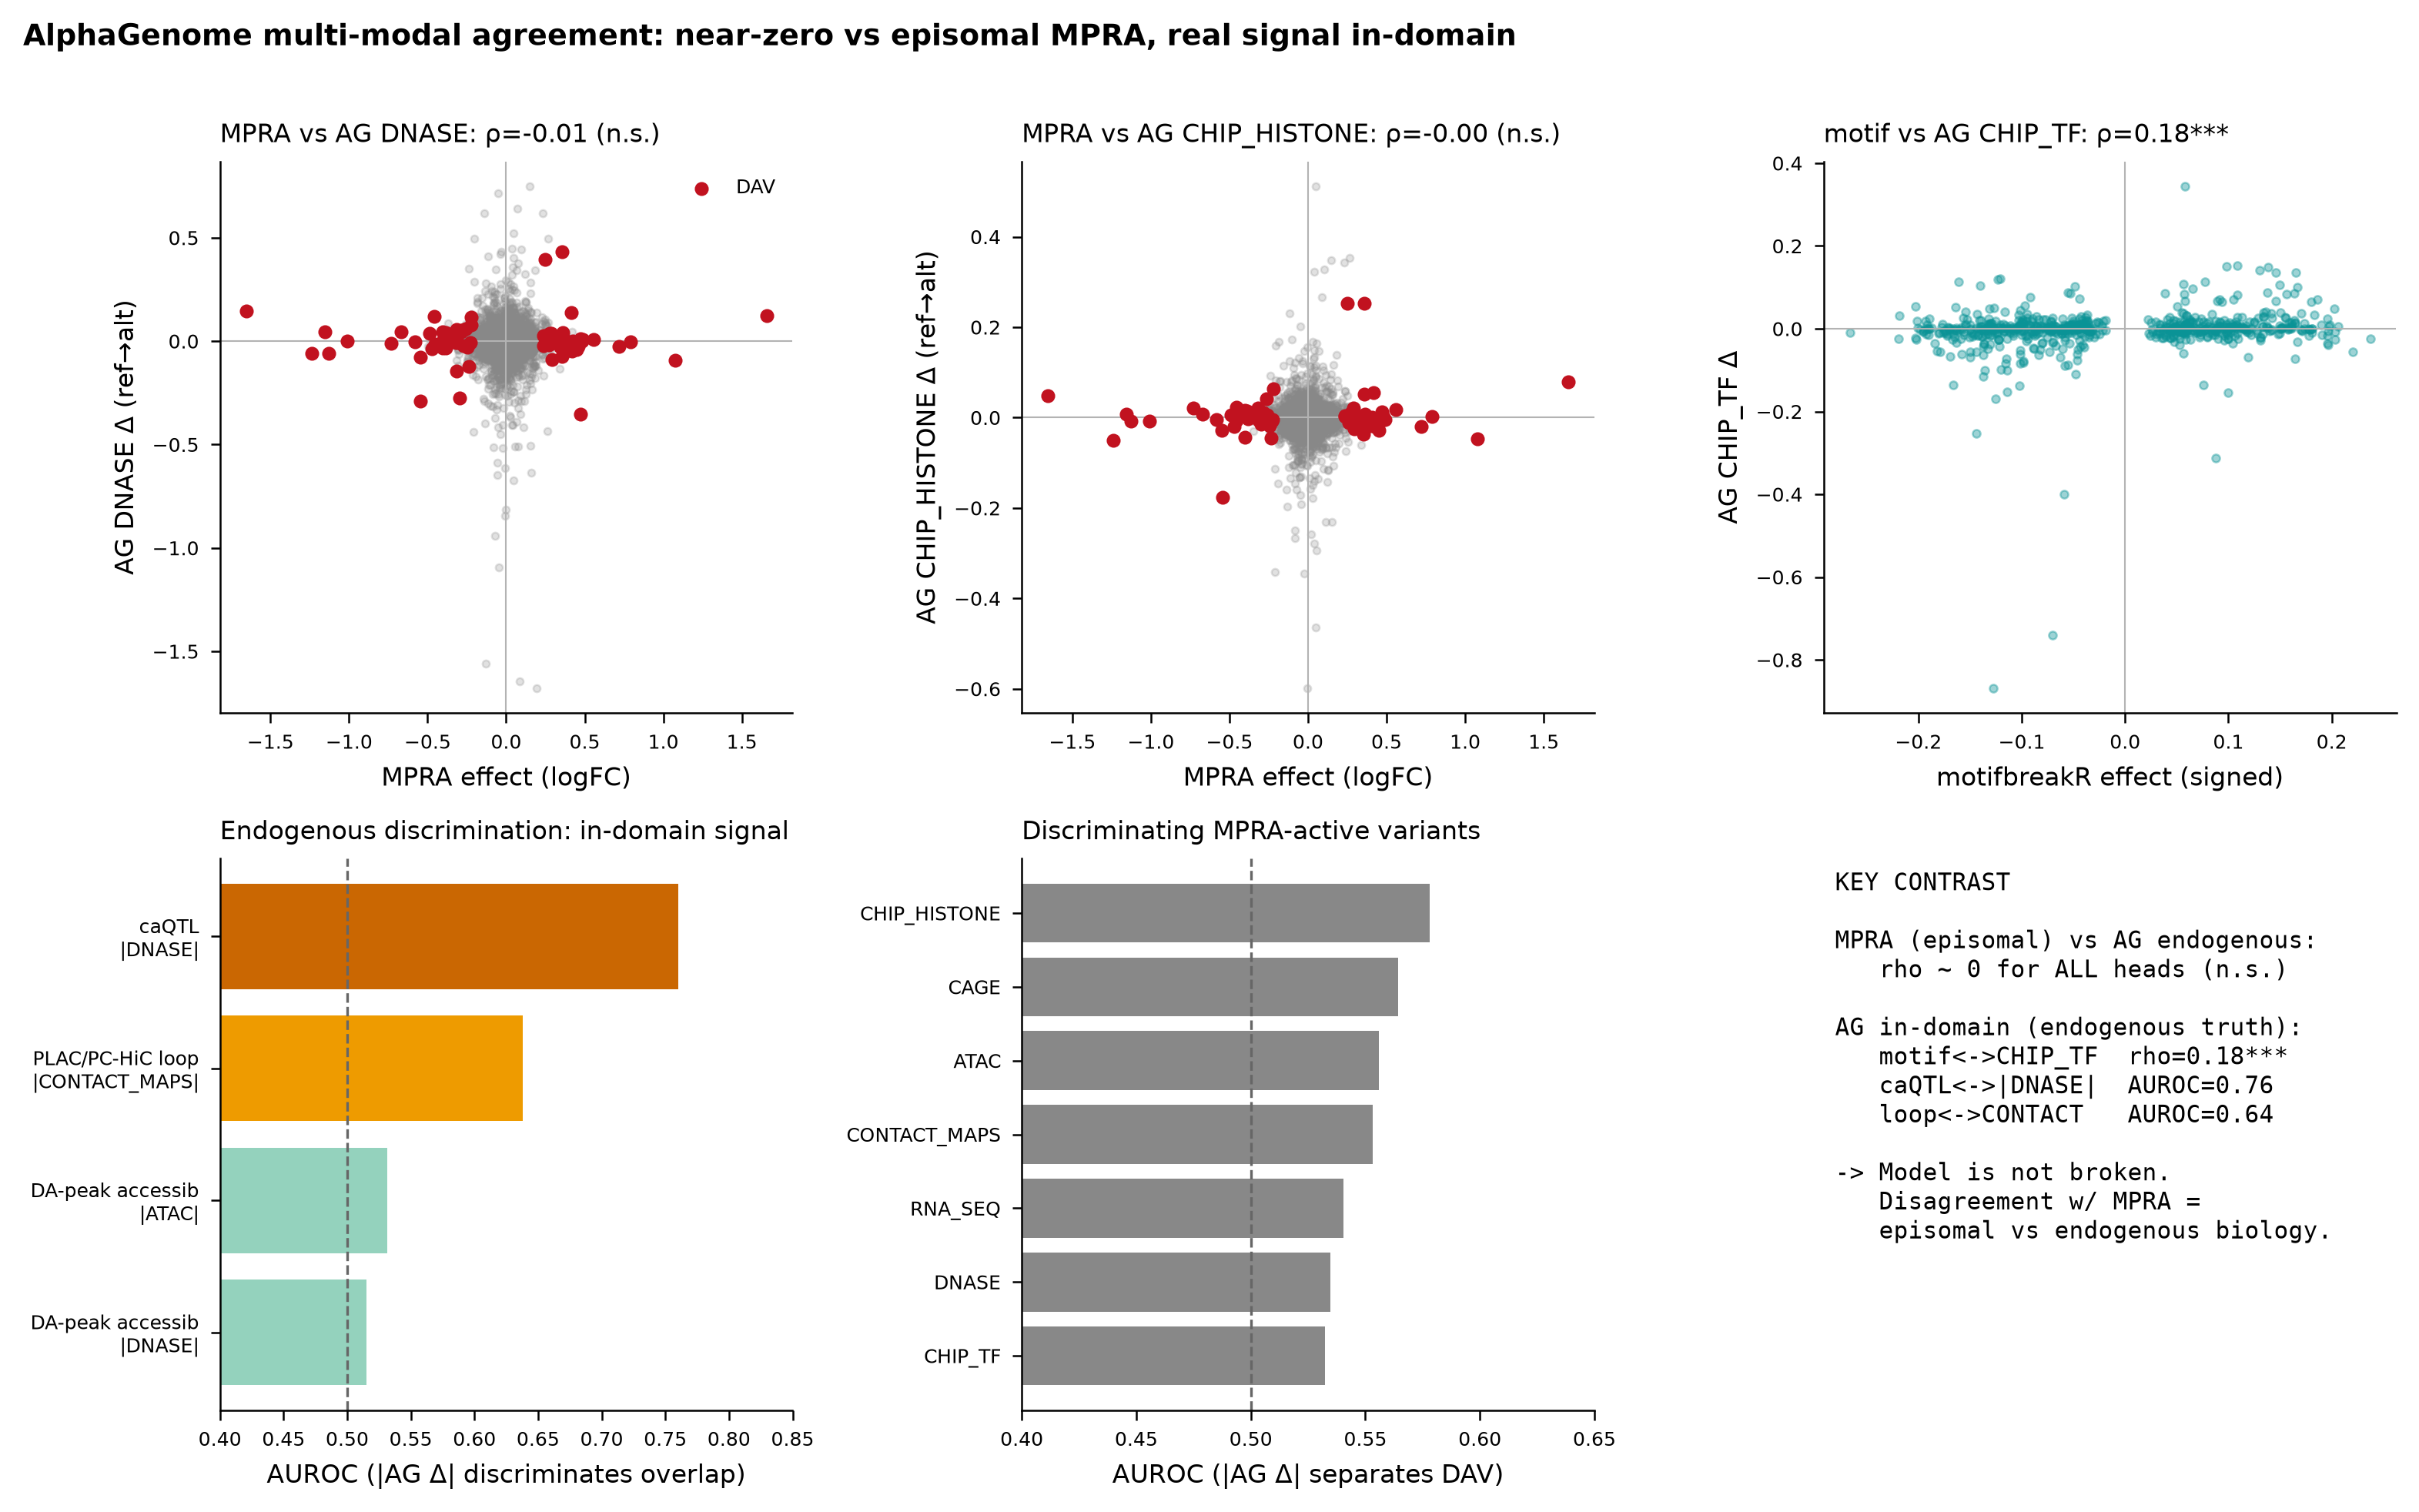
\includegraphics[width=0.49\linewidth]{figures/figS1b.png}
\caption{\textbf{Figure S1. Conservation and multi-modal head robustness} \textbf{(Top)} (a) phyloP conservation by attribution class; model-supported variants are the most conserved (Mann--Whitney p = 0.002). (b) AlphaGenome effect magnitude versus base-level phyloP. \textit{Panel labels retain earlier "verdict" terminology; per the assay-identity correction these classes are read as native-context-dependent vs locally-encoded.} \textbf{(Bottom)} AlphaGenome's seven output heads scored against every measured modality: no head correlates with the lentiMPRA effect, but the ChIP-TF head tracks signed motifbreakR disruption ($\rho$ = 0.18) and the accessibility/contact heads discriminate caQTL overlap (AUROC 0.76) and chromatin loops (AUROC 0.64). \textit{"Episomal" in panel text predates the assay-identity correction and should be read as "integrated reporter."}}
\label{fig:figS1a}
\end{figure*}

\begin{figure*}[t]
\centering
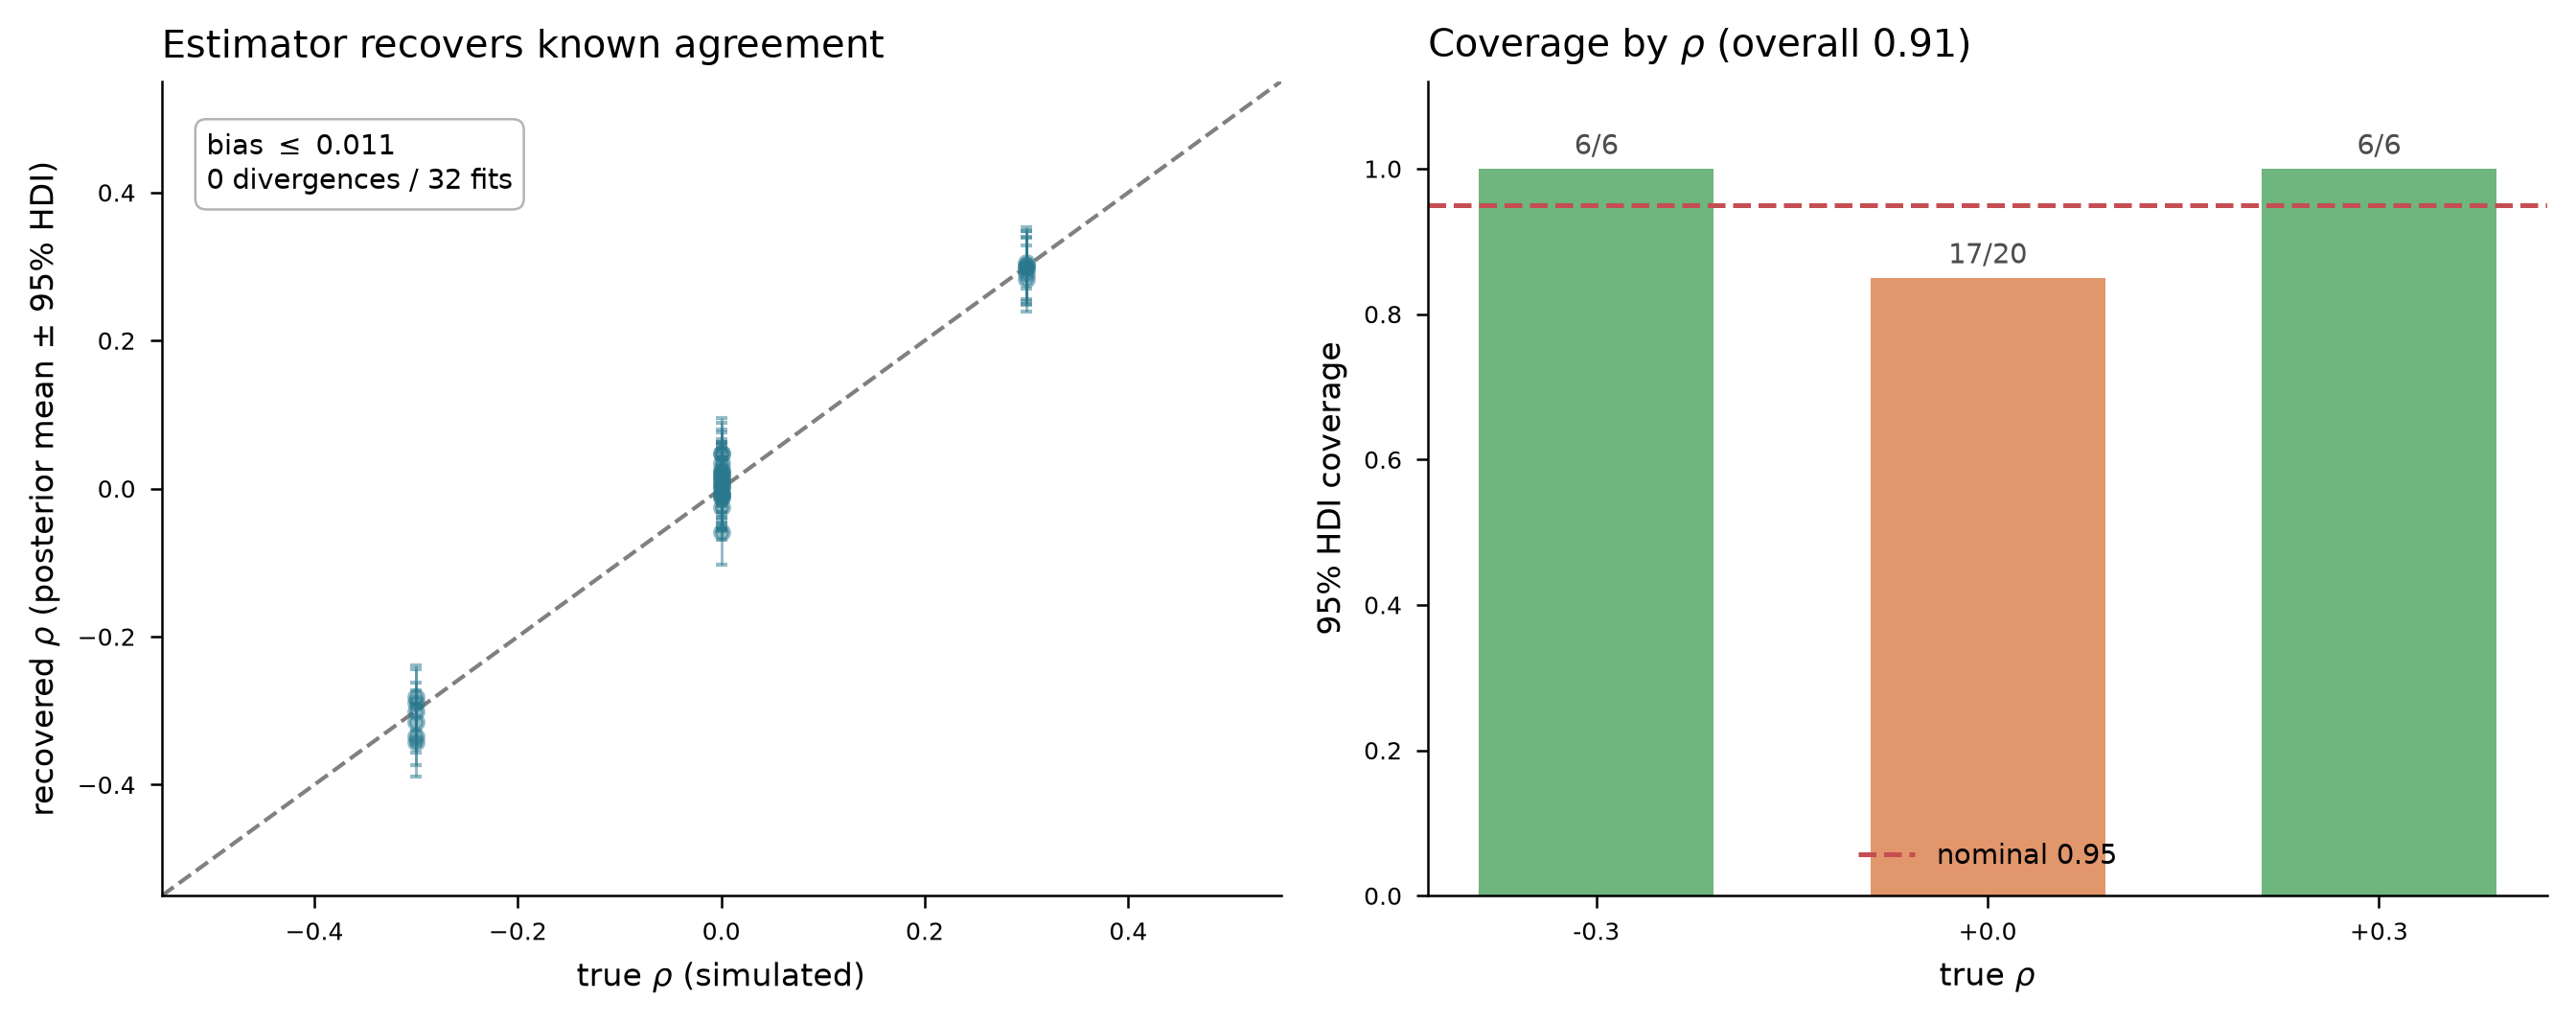
\includegraphics[width=\linewidth]{figures/figS2.png}
\caption{\textbf{Figure S2. Simulation-based calibration of the latent-variable $\rho$ estimator.} Data simulated from the fitted generative model at known $\rho$ (heteroscedastic reporter noise, canonical loadings) and refit; the estimator recovers true $\rho$ with small bias ($\le$ 0.011) and 0 divergences over 32 fits. 95\%-HDI coverage is shown per $\rho$ with fit counts (6/6, 17/20, 6/6; overall 0.91); the $\rho$ = 0 operating point (orange) is replicated 20$\times$ and is within binomial sampling error of the nominal 0.95.}
\label{fig:figS2}
\end{figure*}

\begin{figure*}[t]
\centering
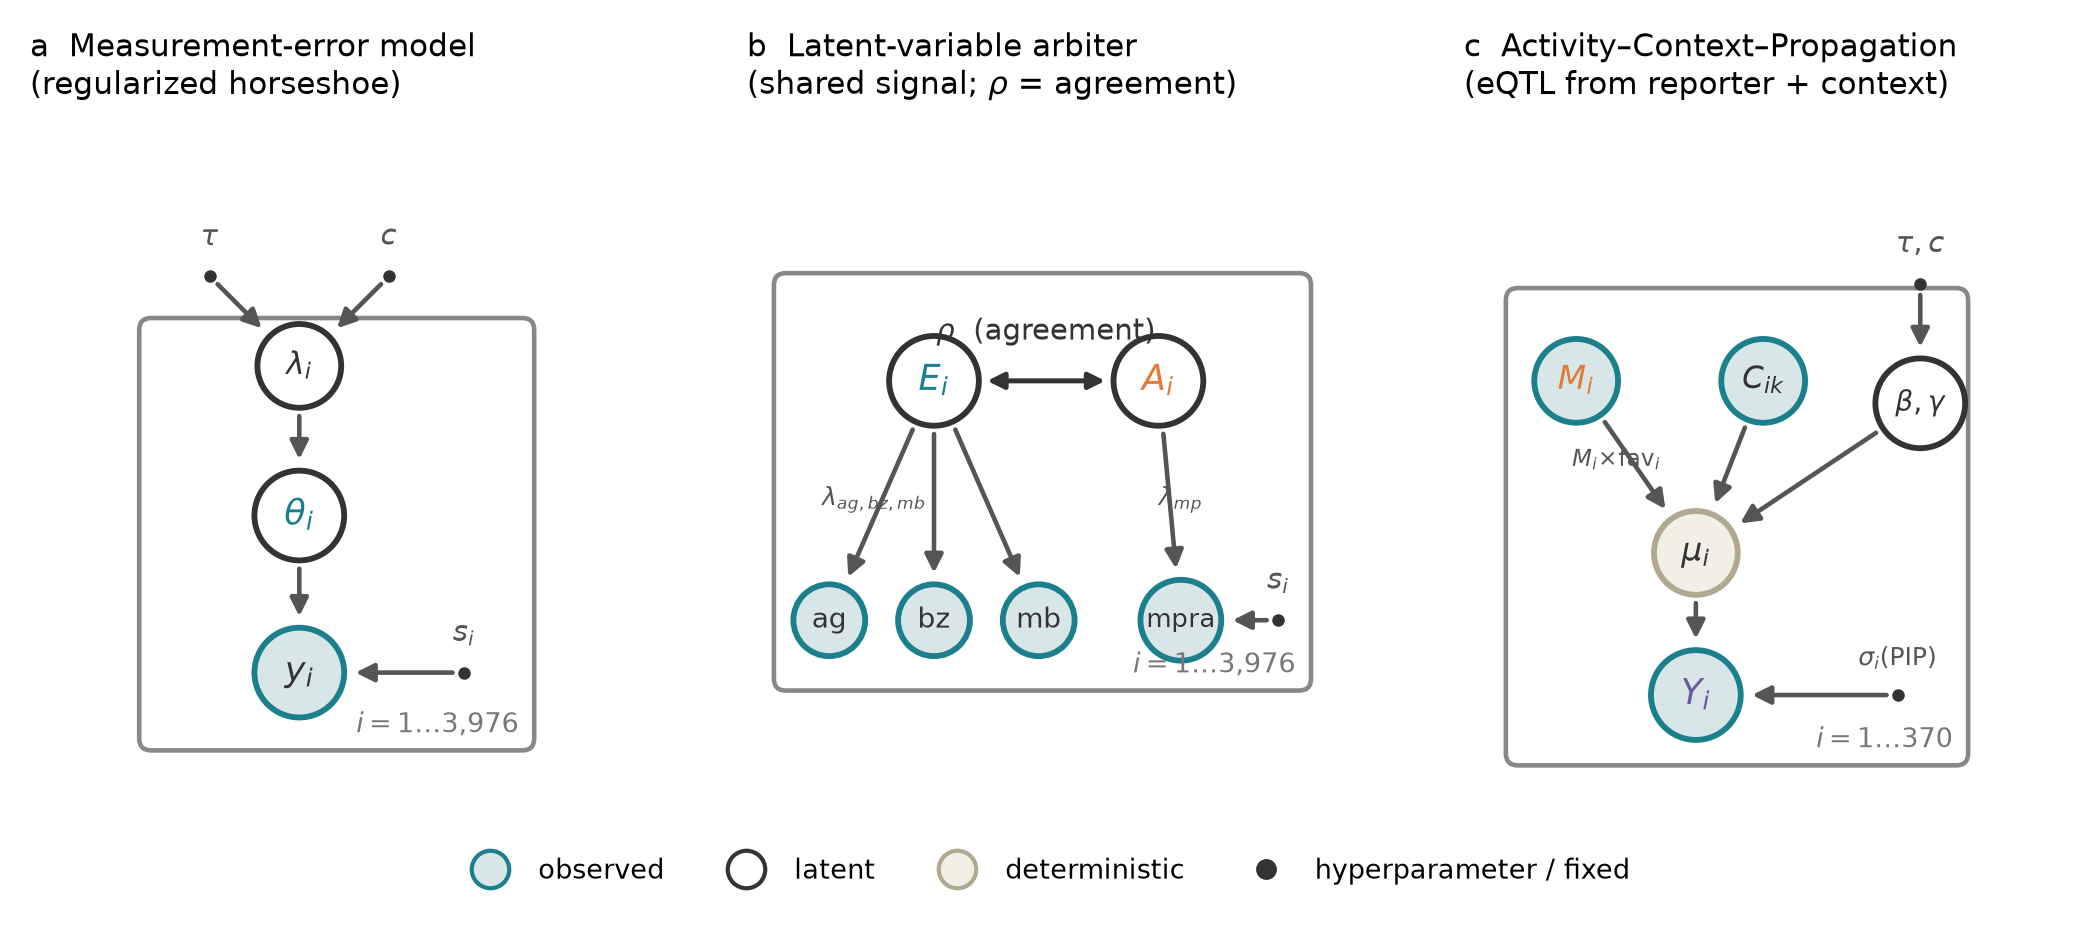
\includegraphics[width=\linewidth]{figures/figS3.png}
\caption{\textbf{Figure S3. Graphical models of the three probabilistic models fit in this study.} Plate notation: shaded nodes are observed, open nodes latent, beige nodes deterministic, and dots fixed hyperparameters or known constants; the outer box is the per-variant plate. (\textbf{a}) Hierarchical measurement-error model: each variant's true effect $\theta$\textsubscript{i} carries a regularized-horseshoe prior (global $\tau$, slab \textit{c}, local $\lambda$\textsubscript{i}) and generates the measured reporter effect y\textsubscript{i} with the known limma standard error s\textsubscript{i} as fixed noise. (\textbf{b}) Latent-variable model: a per-variant endogenous latent E\textsubscript{i} and assay latent A\textsubscript{i} are bivariate-normal with correlation $\rho$, the headline calibrated agreement. AlphaGenome, Borzoi and motifbreakR load on E\textsubscript{i} ($\lambda$\textsubscript{ag,bz,mb}); the lentiMPRA loads on A\textsubscript{i} ($\lambda$\textsubscript{mp}) with heteroscedastic noise s\textsubscript{i}. Per-variant latents are marginalized analytically; $\rho$ is identified through the cross-latent covariance. (\textbf{c}) Activity--Context--Propagation model: the fine-mapped eQTL effect Y\textsubscript{i} is drawn from $\mu$\textsubscript{i} = $\beta$\textsubscript{0} + $\beta$\textsubscript{M}M\textsubscript{i} + $\Sigma$\textsubscript{k}$\beta$\textsubscript{k}C\textsubscript{ik} + $\gamma$(M\textsubscript{i}$\times$fav\textsubscript{i}), regressing the observed reporter effect M\textsubscript{i} and native-context composites C\textsubscript{ik} (plus their interaction) on the endogenous effect, with a regularized-horseshoe prior on context coefficients and a PIP-tempered measurement noise $\sigma$\textsubscript{i}. n = 3,976 for (a,b); n = 370 credible-set variants for (c).}
\label{fig:figS3}
\end{figure*}

\begin{figure*}[t]
\centering
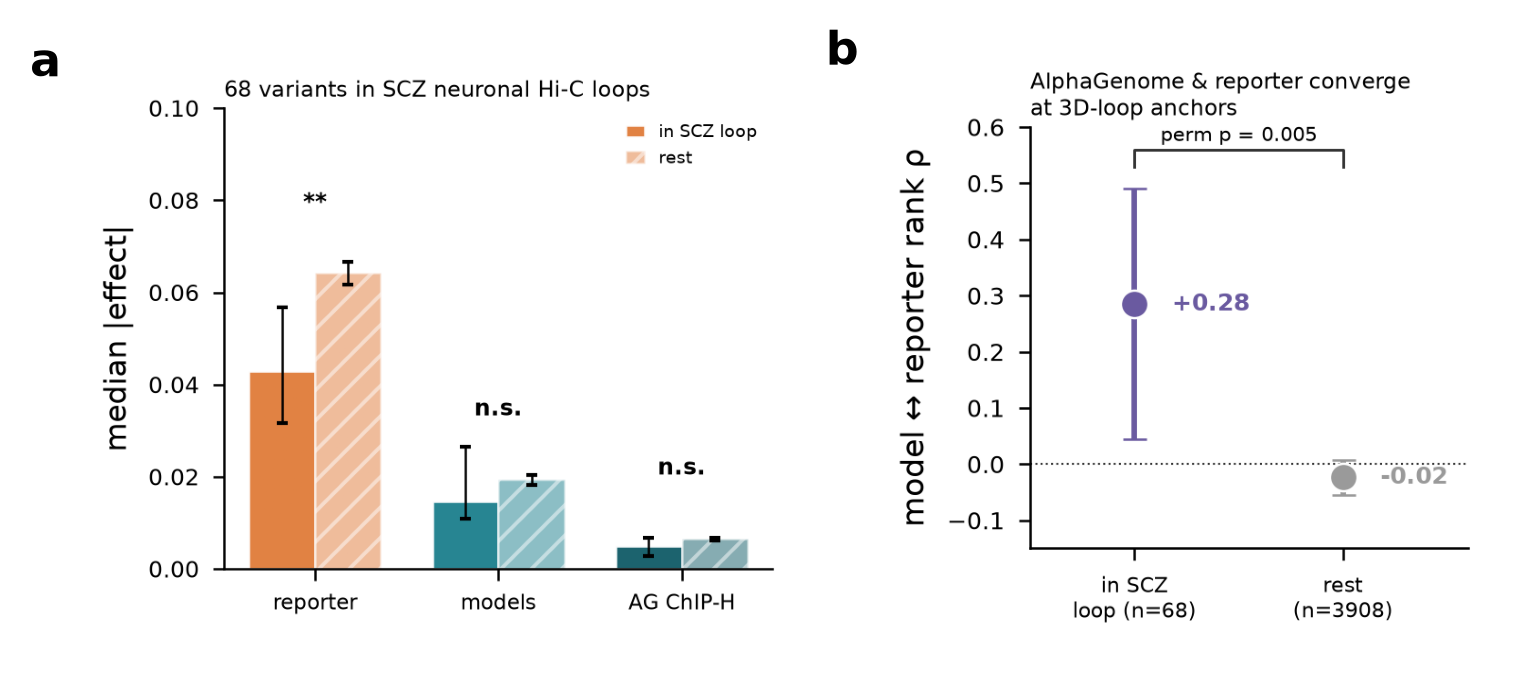
\includegraphics[width=\linewidth]{figures/figS4.png}
\caption{\textbf{Figure S4. Exploratory: model and reporter rankings become more similar at Hi-C loop anchors.} For the 68 of 3,976 variants falling in induced-neuron chromatin-loop anchors (all linkage-disequilibrium proxies, no lead SNPs), the reporter effect is attenuated relative to the rest of the library (median |effect| 0.043 vs 0.064, Mann-Whitney p = 0.007) while the model effect is not (p = 0.32) and baseline activity is matched (p = 0.44); the model-reporter rank correlation rises to $\rho$ = +0.28 (bootstrap 95\% CI [+0.06, +0.48]) versus -0.02 elsewhere (loop-versus-rest permutation p = 0.005). This subgroup is small and defined post hoc; the shift may reflect sequence composition, variant ascertainment, regulatory architecture, or sampling variation, and needs replication in an independent loop dataset. An ectopically integrated reporter does not experience the native loop, so this is not evidence that the two estimands sample the same contact.}
\label{fig:figS4}
\end{figure*}

\begin{figure*}[t]
\centering
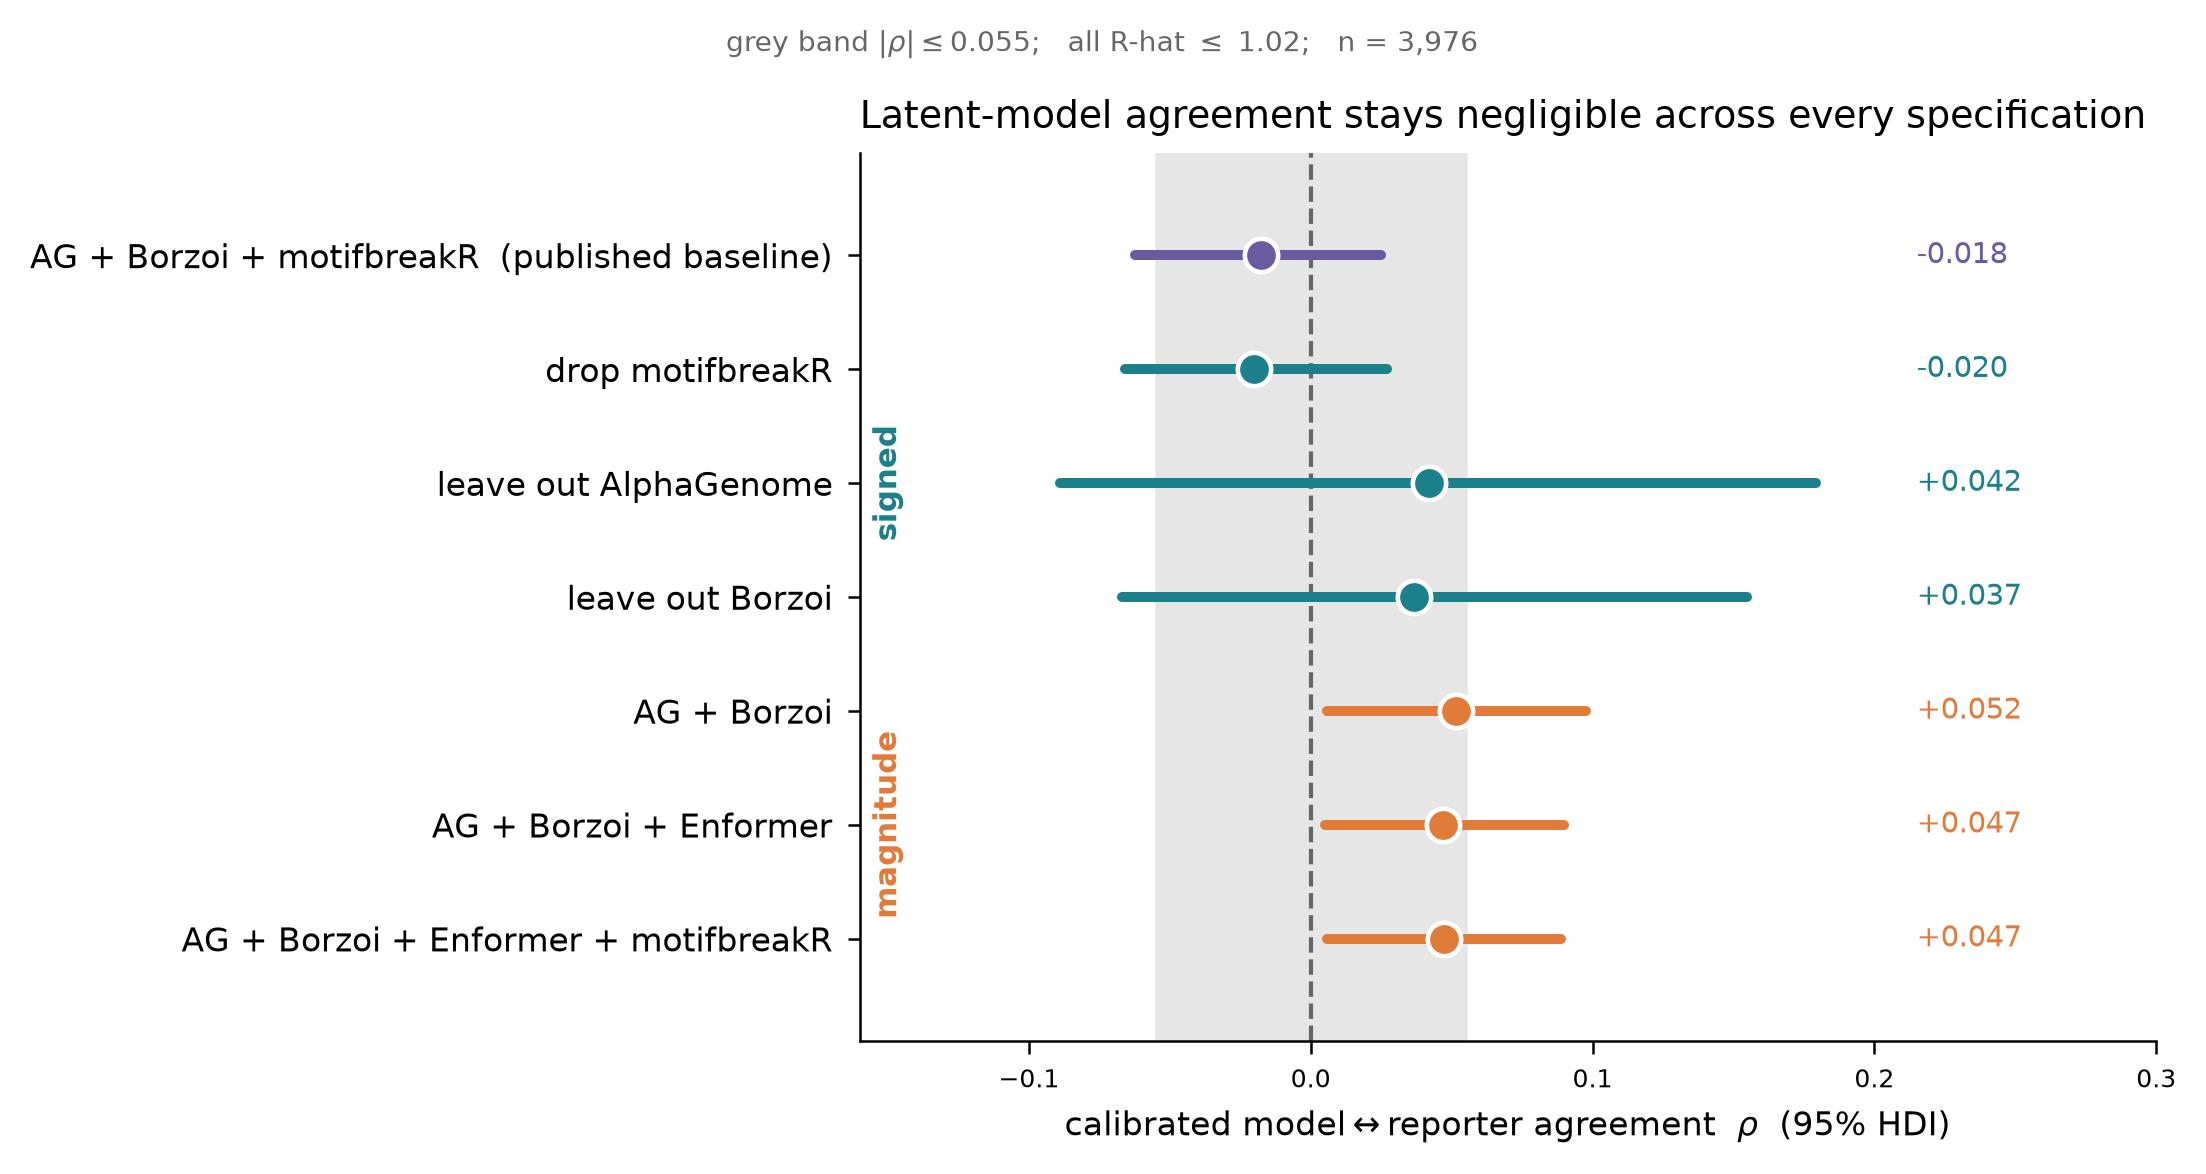
\includegraphics[width=\linewidth]{figures/figS5.png}
\caption{\textbf{Figure S5. The calibrated agreement is robust to model membership and loading choice.} Calibrated model-reporter agreement $\rho$ (posterior mean, 95\% HDI) from the latent-variable model re-fit under seven specifications: the published signed baseline (AlphaGenome + Borzoi + motifbreakR), dropping motifbreakR, leaving out AlphaGenome, leaving out Borzoi, and three magnitude-space fits that add Enformer and motifbreakR. Across all specifications $\rho$ stays within |$\rho$| $\le$ 0.05 (grey band); the signed fits straddle zero and the magnitude fits reach at most $\rho$ = 0.05, a negligible shared effect-size component. All fits converged (R-hat $\le$ 1.02; n = 3,976). Adding a third model, dropping the motif indicator, or removing either CNN does not change the near-zero agreement.}
\label{fig:figS5}
\end{figure*}


\end{document}
